\chapter{Power/EM I} \label{c4_forthchapter:cha}

\section{Electronic Circuits}

\subsection{A basic electronic circuit}

The most basic electronic circuit consist of a power supply (i.e. a battery) that generates an electric potential that aim to move to the ground. And an electrical load (any component consuming electric power) connected to the power supply (Vdd) on one side and to the ``ground" (the reference point from which voltages are measured) on the other side. As the electric potential goes through the load, it (the load) does some kind of a work. We can consider electric current to behave like water, in this example the water wants to go from the mountains (Vdd) to the sea level (Ground) and there are rivers and obstacles that tries to prevent it to do so. When the load has small resistance then more of the current will “flow” through it, and when the load has bigger resistance then the “flow” is smaller.

There are two different ways in which we can wire things together in an electric circuit, called series and parallel. When things are wired in series, things are wired one after another, such that electricity has to pass through one load, then the next load, then the next, and so on. When things are wired in parallel, they are wired side by side, such that electricity passes through all of them at the same time, from one common point to another common point. The difference in the electric potential between the power supply and the ground creates an electric current which flows through the load toward the ground. The difference in electric potential between two points is measured in Volts (usually denoted by \textbf{\textit{V}}). The amount of current flowing through the circuit at a given time is measured in Amperes (denoted by \textbf{\textit{A}}). The electrical resistance of the load is a measure of its opposition to the flow of electric current through it. It is measured in Ohms (and denoted by \textbf{\textit{R}}).

\subsection{Resistors}

As the name implies, a resistor resists the flow of electrical current. The amount of resistance is measured in Ohms. A resistor is considered a passive component that consumes power that is dissipated as heat. The power rating of a resistor determines how much power it can consume without overheating.

\begin{figure}[!ht]
    \centering
    \tikzset{every picture/.style={line width=0.75pt}} %set default line width to 0.75pt        

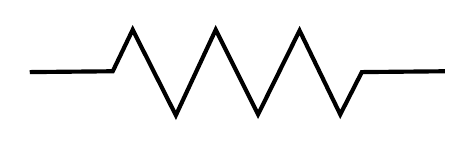
\begin{tikzpicture}[x=0.75pt,y=0.75pt,yscale=-1,xscale=1]
%uncomment if require: \path (0,82); %set diagram left start at 0, and has height of 82

%Straight Lines [id:da11666992549989796] 
\draw [line width=1.5]    (11.4,40.02) -- (51.4,39.62) -- (61,19.62) -- (81.8,60.82) -- (101,19.62) -- (121.4,60.42) -- (141.4,20.02) -- (161,60.42) -- (171.4,40.02) -- (211.4,39.62) ;






\end{tikzpicture}
    \caption{Resistor Symbol in Circuit Diagrams.} \label{fig:resistor}
\end{figure}

\subsection{Ohm's law}

\begin{figure}[!ht]
	\centering
	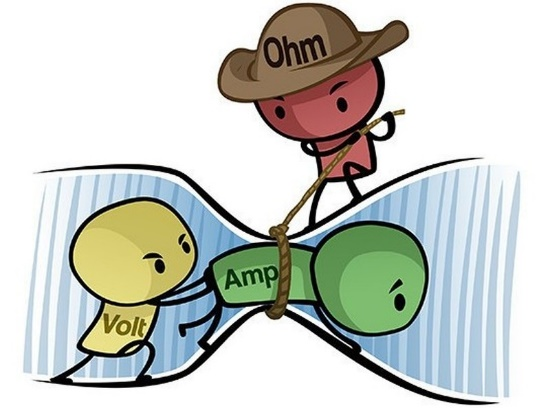
\includegraphics{images/ohms_law_cartoon.png}
	\caption{Ohm's Law.} \label{fig:ohms_law_cartoon}
\end{figure}

Ohm's law defines the relationship between the Voltage, Current and Resistance in a circuit: The voltage is equal to the current multiplied by the resistance of the load. 

\begin{displaymath}\label{eq:ohm}
    V=I*R
\end{displaymath}

Since in most of the circuits we are using, the voltage is fixed (defined by the characteristics of the power supply), a change in the resistance of the circuit will cause a change in the current in the opposite direction. This means we can measure the current over time in order to calculate the resistance. A useful analogy for the relations between V, I and R is to imagine a fountain on a high mountain, where the water flow down through a river to the sea. The difference in height between the fountain and the sea is the Voltage, the width of the river can be thought of as the resistance, and the flow of the water is the current.

\subsection{Power}

Power is the rate at which work is done by the circuit and is measured in Watts. Electricity bills are measured by K Watts hour, i.e. 1 KWH is 1 kilo watts used over an hour, and this is the energy that we used and we need to pay for. $Power = Work / Time$

\begin{displaymath}\label{eq:power_consumption}
    \textrm{Power consumption:} P=I*V
\end{displaymath}

For example we can take a look on a phone; the battery can be measure in Milliamper hour, i.e. if the battery is 3000mil Amper Hour so if the current is 1 Amper then we can use it for 3 hours. If we want the battery to run out quickly, we can use services like streaming, flashlight and more. That means we have greater current that caused by leveraging the load of the phone and the battery will run our much faster than before. The phone also, will get hot. If a device is getting hot then it sometimes uses its fans (noise), and so we can detect it for cyber usage.

Electricity can be used to do various kinds of work:
\begin{itemize}
    \item Electromagnetic work (light a bulb, transmit a Wi-Fi signal)
    \item Thermal work (heating)
    \item Mechanical work (spin a motor, vibrate a speaker)
    \item Chemical work (charging a battery)
    \item Computational work (store or load from memory, compute a value)
\end{itemize}

\subsection{Power Consumption}

When the current leaves the circuit to the ground then we consume it as power, but sometimes we need to be careful as there are cases where the current is no leaving the circuit, like battery charging. In order to measure the power we will connect our measuring device between the load and the ground. The power consumption of a device is the work it does divided by time. It is measured in Watts (\textbf{\textit{W}}). The power consumption can be calculated as current (\textbf{\textit{I}}) multiplied by Voltage (\textbf{\textit{V}}).

\subsection{Current and Voltage dividers}

Before we take a look at two simple electronic circuits, we need to introduce two additional terms:
A \textbf{short (closed) circuit} is a piece of wire with almost no resistance at all. The circuit is in a closed state and there is current in the circuit. In other words, it works as normal.
An \textbf{open circuit} is a circuit which doesn't allow any current to pass through it. The circuit is in an open state and there is no current in the circuit; that's to say. It doesn't work.

\begin{figure}[!ht]
    \centering
    

\tikzset{every picture/.style={line width=0.75pt}} %set default line width to 0.75pt        

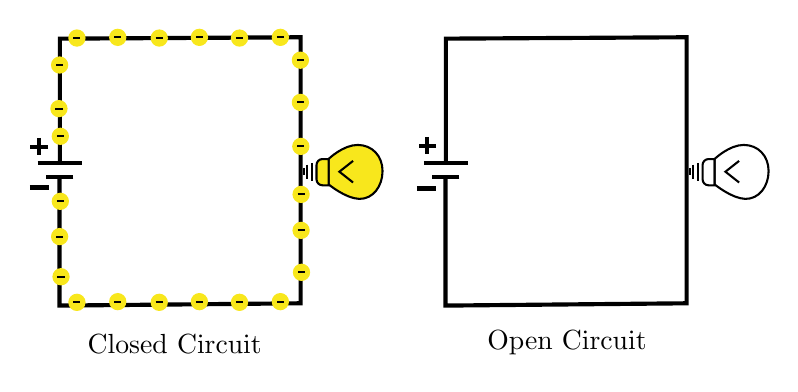
\begin{tikzpicture}[x=0.75pt,y=0.75pt,yscale=-1,xscale=1]
%uncomment if require: \path (0,199.3333282470703); %set diagram left start at 0, and has height of 199.3333282470703

%Straight Lines [id:da2325261898014528] 
\draw [color={rgb, 255:red, 0; green, 0; blue, 0 }  ,draw opacity=1 ][line width=1.5]    (35.5,90.67) -- (35.5,152.67) -- (151.67,151.56) -- (151.67,23.39) -- (35.67,24.06) -- (35.67,84.06) ;

\draw [shift={(35.5,90.67)}, rotate = 270] [color={rgb, 255:red, 0; green, 0; blue, 0 }  ,draw opacity=1 ][line width=1.5]    (0,6.71) -- (0,-6.71)   ;
%Straight Lines [id:da28409341931115617] 
\draw [color={rgb, 255:red, 0; green, 0; blue, 0 }  ,draw opacity=1 ][line width=1.5]    (25,84.06) -- (46.33,84.06) ;


%Shape: Polygon Curved [id:ds5857087256403513] 
\draw  [fill={rgb, 255:red, 248; green, 231; blue, 28 }  ,fill opacity=1 ] (165.14,94.26) .. controls (165.14,94.26) and (173.39,101.09) .. (179.94,101.26) .. controls (186.5,101.42) and (191.14,95.16) .. (191.14,87.86) .. controls (191.15,80.56) and (186.14,75.26) .. (179.14,75.26) .. controls (172.14,75.26) and (165.12,82.03) .. (165.14,82.06) .. controls (165.17,82.08) and (165.14,94.26) .. (165.14,94.26) -- cycle ;
%Rounded Same Side Corner Rect [id:dp42554815939285007] 
\draw  [fill={rgb, 255:red, 248; green, 231; blue, 28 }  ,fill opacity=1 ] (162.24,94.72) .. controls (160.63,94.72) and (159.33,93.42) .. (159.33,91.82) -- (159.33,84.96) .. controls (159.33,83.36) and (160.63,82.06) .. (162.24,82.06) -- (165.14,82.06) .. controls (165.14,82.06) and (165.14,82.06) .. (165.14,82.06) -- (165.14,94.72) .. controls (165.14,94.72) and (165.14,94.72) .. (165.14,94.72) -- cycle ;
%Straight Lines [id:da9150604099279609] 
\draw [line width=0.75]    (156.94,83.96) -- (156.94,92.56) ;


%Straight Lines [id:da28384528220983696] 
\draw [line width=0.75]    (154.94,84.76) -- (154.94,91.56) ;


%Straight Lines [id:da8752324892632142] 
\draw [line width=0.75]    (153.34,86.36) -- (153.34,89.56) ;


%Straight Lines [id:da25290786107493535] 
\draw [line width=0.75]    (176.94,82.96) -- (170.34,88.16) -- (176.94,93.36) ;


%Straight Lines [id:da9185196513242853] 
\draw [line width=1.5]    (21.17,95.78) -- (30.5,95.78) ;


%Shape: Circle [id:dp23397738064818174] 
\draw  [draw opacity=0][fill={rgb, 255:red, 248; green, 231; blue, 28 }  ,fill opacity=1 ] (147.6,75.97) .. controls (147.6,73.67) and (149.47,71.8) .. (151.77,71.8) .. controls (154.07,71.8) and (155.93,73.67) .. (155.93,75.97) .. controls (155.93,78.27) and (154.07,80.13) .. (151.77,80.13) .. controls (149.47,80.13) and (147.6,78.27) .. (147.6,75.97) -- cycle ;
%Straight Lines [id:da482836286674198] 
\draw    (150.05,75.97) -- (153.48,75.97) ;



%Shape: Circle [id:dp7549375095754003] 
\draw  [draw opacity=0][fill={rgb, 255:red, 248; green, 231; blue, 28 }  ,fill opacity=1 ] (147.4,54.77) .. controls (147.4,52.47) and (149.27,50.6) .. (151.57,50.6) .. controls (153.87,50.6) and (155.73,52.47) .. (155.73,54.77) .. controls (155.73,57.07) and (153.87,58.93) .. (151.57,58.93) .. controls (149.27,58.93) and (147.4,57.07) .. (147.4,54.77) -- cycle ;
%Straight Lines [id:da4285424058101477] 
\draw    (149.85,54.77) -- (153.28,54.77) ;



%Shape: Circle [id:dp5457818708688953] 
\draw  [draw opacity=0][fill={rgb, 255:red, 248; green, 231; blue, 28 }  ,fill opacity=1 ] (147.4,34.43) .. controls (147.4,32.13) and (149.27,30.27) .. (151.57,30.27) .. controls (153.87,30.27) and (155.73,32.13) .. (155.73,34.43) .. controls (155.73,36.73) and (153.87,38.6) .. (151.57,38.6) .. controls (149.27,38.6) and (147.4,36.73) .. (147.4,34.43) -- cycle ;
%Straight Lines [id:da8515924061724973] 
\draw    (149.85,34.43) -- (153.28,34.43) ;



%Shape: Circle [id:dp4359422667224846] 
\draw  [draw opacity=0][fill={rgb, 255:red, 248; green, 231; blue, 28 }  ,fill opacity=1 ] (137.73,23.43) .. controls (137.73,21.13) and (139.6,19.27) .. (141.9,19.27) .. controls (144.2,19.27) and (146.07,21.13) .. (146.07,23.43) .. controls (146.07,25.73) and (144.2,27.6) .. (141.9,27.6) .. controls (139.6,27.6) and (137.73,25.73) .. (137.73,23.43) -- cycle ;
%Straight Lines [id:da45892746068057066] 
\draw    (140.19,23.43) -- (143.61,23.43) ;



%Shape: Circle [id:dp10968014625901534] 
\draw  [draw opacity=0][fill={rgb, 255:red, 248; green, 231; blue, 28 }  ,fill opacity=1 ] (118.07,23.77) .. controls (118.07,21.47) and (119.93,19.6) .. (122.23,19.6) .. controls (124.53,19.6) and (126.4,21.47) .. (126.4,23.77) .. controls (126.4,26.07) and (124.53,27.93) .. (122.23,27.93) .. controls (119.93,27.93) and (118.07,26.07) .. (118.07,23.77) -- cycle ;
%Straight Lines [id:da5692830288753206] 
\draw    (120.52,23.77) -- (123.95,23.77) ;



%Shape: Circle [id:dp43116716627713836] 
\draw  [draw opacity=0][fill={rgb, 255:red, 248; green, 231; blue, 28 }  ,fill opacity=1 ] (98.73,23.43) .. controls (98.73,21.13) and (100.6,19.27) .. (102.9,19.27) .. controls (105.2,19.27) and (107.07,21.13) .. (107.07,23.43) .. controls (107.07,25.73) and (105.2,27.6) .. (102.9,27.6) .. controls (100.6,27.6) and (98.73,25.73) .. (98.73,23.43) -- cycle ;
%Straight Lines [id:da7403562369362462] 
\draw    (101.19,23.43) -- (104.61,23.43) ;



%Shape: Circle [id:dp03302036024104882] 
\draw  [draw opacity=0][fill={rgb, 255:red, 248; green, 231; blue, 28 }  ,fill opacity=1 ] (79.4,23.77) .. controls (79.4,21.47) and (81.27,19.6) .. (83.57,19.6) .. controls (85.87,19.6) and (87.73,21.47) .. (87.73,23.77) .. controls (87.73,26.07) and (85.87,27.93) .. (83.57,27.93) .. controls (81.27,27.93) and (79.4,26.07) .. (79.4,23.77) -- cycle ;
%Straight Lines [id:da40757318650872465] 
\draw    (81.85,23.77) -- (85.28,23.77) ;



%Shape: Circle [id:dp8000122366529838] 
\draw  [draw opacity=0][fill={rgb, 255:red, 248; green, 231; blue, 28 }  ,fill opacity=1 ] (59.4,23.43) .. controls (59.4,21.13) and (61.27,19.27) .. (63.57,19.27) .. controls (65.87,19.27) and (67.73,21.13) .. (67.73,23.43) .. controls (67.73,25.73) and (65.87,27.6) .. (63.57,27.6) .. controls (61.27,27.6) and (59.4,25.73) .. (59.4,23.43) -- cycle ;
%Straight Lines [id:da0875021467717878] 
\draw    (61.85,23.43) -- (65.28,23.43) ;



%Shape: Circle [id:dp05690070919084467] 
\draw  [draw opacity=0][fill={rgb, 255:red, 248; green, 231; blue, 28 }  ,fill opacity=1 ] (39.73,23.77) .. controls (39.73,21.47) and (41.6,19.6) .. (43.9,19.6) .. controls (46.2,19.6) and (48.07,21.47) .. (48.07,23.77) .. controls (48.07,26.07) and (46.2,27.93) .. (43.9,27.93) .. controls (41.6,27.93) and (39.73,26.07) .. (39.73,23.77) -- cycle ;
%Straight Lines [id:da5744558280008554] 
\draw    (42.19,23.77) -- (45.61,23.77) ;



%Shape: Circle [id:dp09815936705452866] 
\draw  [draw opacity=0][fill={rgb, 255:red, 248; green, 231; blue, 28 }  ,fill opacity=1 ] (31.4,36.77) .. controls (31.4,34.47) and (33.27,32.6) .. (35.57,32.6) .. controls (37.87,32.6) and (39.73,34.47) .. (39.73,36.77) .. controls (39.73,39.07) and (37.87,40.93) .. (35.57,40.93) .. controls (33.27,40.93) and (31.4,39.07) .. (31.4,36.77) -- cycle ;
%Straight Lines [id:da1455188221370589] 
\draw    (33.85,36.77) -- (37.28,36.77) ;



%Shape: Circle [id:dp898572524230915] 
\draw  [draw opacity=0][fill={rgb, 255:red, 248; green, 231; blue, 28 }  ,fill opacity=1 ] (31.07,57.77) .. controls (31.07,55.47) and (32.93,53.6) .. (35.23,53.6) .. controls (37.53,53.6) and (39.4,55.47) .. (39.4,57.77) .. controls (39.4,60.07) and (37.53,61.93) .. (35.23,61.93) .. controls (32.93,61.93) and (31.07,60.07) .. (31.07,57.77) -- cycle ;
%Straight Lines [id:da9743601868292349] 
\draw    (33.52,57.77) -- (36.95,57.77) ;



%Shape: Circle [id:dp6955964743895362] 
\draw  [draw opacity=0][fill={rgb, 255:red, 248; green, 231; blue, 28 }  ,fill opacity=1 ] (31.73,71.1) .. controls (31.73,68.8) and (33.6,66.93) .. (35.9,66.93) .. controls (38.2,66.93) and (40.07,68.8) .. (40.07,71.1) .. controls (40.07,73.4) and (38.2,75.27) .. (35.9,75.27) .. controls (33.6,75.27) and (31.73,73.4) .. (31.73,71.1) -- cycle ;
%Straight Lines [id:da6213610339187869] 
\draw    (34.19,71.1) -- (37.61,71.1) ;



%Shape: Circle [id:dp9264817359074005] 
\draw  [draw opacity=0][fill={rgb, 255:red, 248; green, 231; blue, 28 }  ,fill opacity=1 ] (137.73,150.77) .. controls (137.73,148.47) and (139.6,146.6) .. (141.9,146.6) .. controls (144.2,146.6) and (146.07,148.47) .. (146.07,150.77) .. controls (146.07,153.07) and (144.2,154.93) .. (141.9,154.93) .. controls (139.6,154.93) and (137.73,153.07) .. (137.73,150.77) -- cycle ;
%Straight Lines [id:da9036669479861532] 
\draw    (140.19,150.77) -- (143.61,150.77) ;



%Shape: Circle [id:dp5844969098724175] 
\draw  [draw opacity=0][fill={rgb, 255:red, 248; green, 231; blue, 28 }  ,fill opacity=1 ] (118.07,151.1) .. controls (118.07,148.8) and (119.93,146.93) .. (122.23,146.93) .. controls (124.53,146.93) and (126.4,148.8) .. (126.4,151.1) .. controls (126.4,153.4) and (124.53,155.27) .. (122.23,155.27) .. controls (119.93,155.27) and (118.07,153.4) .. (118.07,151.1) -- cycle ;
%Straight Lines [id:da09046684668382188] 
\draw    (120.52,151.1) -- (123.95,151.1) ;



%Shape: Circle [id:dp3885888198313816] 
\draw  [draw opacity=0][fill={rgb, 255:red, 248; green, 231; blue, 28 }  ,fill opacity=1 ] (98.73,150.77) .. controls (98.73,148.47) and (100.6,146.6) .. (102.9,146.6) .. controls (105.2,146.6) and (107.07,148.47) .. (107.07,150.77) .. controls (107.07,153.07) and (105.2,154.93) .. (102.9,154.93) .. controls (100.6,154.93) and (98.73,153.07) .. (98.73,150.77) -- cycle ;
%Straight Lines [id:da7589232460632716] 
\draw    (101.19,150.77) -- (104.61,150.77) ;



%Shape: Circle [id:dp8123284122535401] 
\draw  [draw opacity=0][fill={rgb, 255:red, 248; green, 231; blue, 28 }  ,fill opacity=1 ] (79.4,151.1) .. controls (79.4,148.8) and (81.27,146.93) .. (83.57,146.93) .. controls (85.87,146.93) and (87.73,148.8) .. (87.73,151.1) .. controls (87.73,153.4) and (85.87,155.27) .. (83.57,155.27) .. controls (81.27,155.27) and (79.4,153.4) .. (79.4,151.1) -- cycle ;
%Straight Lines [id:da22457079830109827] 
\draw    (81.85,151.1) -- (85.28,151.1) ;



%Shape: Circle [id:dp3398253087803511] 
\draw  [draw opacity=0][fill={rgb, 255:red, 248; green, 231; blue, 28 }  ,fill opacity=1 ] (59.4,150.77) .. controls (59.4,148.47) and (61.27,146.6) .. (63.57,146.6) .. controls (65.87,146.6) and (67.73,148.47) .. (67.73,150.77) .. controls (67.73,153.07) and (65.87,154.93) .. (63.57,154.93) .. controls (61.27,154.93) and (59.4,153.07) .. (59.4,150.77) -- cycle ;
%Straight Lines [id:da4761807980612174] 
\draw    (61.85,150.77) -- (65.28,150.77) ;



%Shape: Circle [id:dp08104931167537988] 
\draw  [draw opacity=0][fill={rgb, 255:red, 248; green, 231; blue, 28 }  ,fill opacity=1 ] (39.73,151.1) .. controls (39.73,148.8) and (41.6,146.93) .. (43.9,146.93) .. controls (46.2,146.93) and (48.07,148.8) .. (48.07,151.1) .. controls (48.07,153.4) and (46.2,155.27) .. (43.9,155.27) .. controls (41.6,155.27) and (39.73,153.4) .. (39.73,151.1) -- cycle ;
%Straight Lines [id:da9286267104864216] 
\draw    (42.19,151.1) -- (45.61,151.1) ;



%Shape: Circle [id:dp4591909478978906] 
\draw  [draw opacity=0][fill={rgb, 255:red, 248; green, 231; blue, 28 }  ,fill opacity=1 ] (147.93,136.63) .. controls (147.93,134.33) and (149.8,132.47) .. (152.1,132.47) .. controls (154.4,132.47) and (156.27,134.33) .. (156.27,136.63) .. controls (156.27,138.93) and (154.4,140.8) .. (152.1,140.8) .. controls (149.8,140.8) and (147.93,138.93) .. (147.93,136.63) -- cycle ;
%Straight Lines [id:da27768924319706034] 
\draw    (150.39,136.63) -- (153.81,136.63) ;



%Shape: Circle [id:dp49148284196801884] 
\draw  [draw opacity=0][fill={rgb, 255:red, 248; green, 231; blue, 28 }  ,fill opacity=1 ] (147.73,116.43) .. controls (147.73,114.13) and (149.6,112.27) .. (151.9,112.27) .. controls (154.2,112.27) and (156.07,114.13) .. (156.07,116.43) .. controls (156.07,118.73) and (154.2,120.6) .. (151.9,120.6) .. controls (149.6,120.6) and (147.73,118.73) .. (147.73,116.43) -- cycle ;
%Straight Lines [id:da43922422127862903] 
\draw    (150.19,116.43) -- (153.61,116.43) ;



%Shape: Circle [id:dp45434208681679933] 
\draw  [draw opacity=0][fill={rgb, 255:red, 248; green, 231; blue, 28 }  ,fill opacity=1 ] (147.73,99.1) .. controls (147.73,96.8) and (149.6,94.93) .. (151.9,94.93) .. controls (154.2,94.93) and (156.07,96.8) .. (156.07,99.1) .. controls (156.07,101.4) and (154.2,103.27) .. (151.9,103.27) .. controls (149.6,103.27) and (147.73,101.4) .. (147.73,99.1) -- cycle ;
%Straight Lines [id:da5414882082978889] 
\draw    (150.19,99.1) -- (153.61,99.1) ;



%Shape: Circle [id:dp3331602882322313] 
\draw  [draw opacity=0][fill={rgb, 255:red, 248; green, 231; blue, 28 }  ,fill opacity=1 ] (31.73,102.43) .. controls (31.73,100.13) and (33.6,98.27) .. (35.9,98.27) .. controls (38.2,98.27) and (40.07,100.13) .. (40.07,102.43) .. controls (40.07,104.73) and (38.2,106.6) .. (35.9,106.6) .. controls (33.6,106.6) and (31.73,104.73) .. (31.73,102.43) -- cycle ;
%Straight Lines [id:da02142976481388592] 
\draw    (34.19,102.43) -- (37.61,102.43) ;



%Shape: Circle [id:dp9754321905396712] 
\draw  [draw opacity=0][fill={rgb, 255:red, 248; green, 231; blue, 28 }  ,fill opacity=1 ] (31.4,119.43) .. controls (31.4,117.13) and (33.27,115.27) .. (35.57,115.27) .. controls (37.87,115.27) and (39.73,117.13) .. (39.73,119.43) .. controls (39.73,121.73) and (37.87,123.6) .. (35.57,123.6) .. controls (33.27,123.6) and (31.4,121.73) .. (31.4,119.43) -- cycle ;
%Straight Lines [id:da7550329579379682] 
\draw    (33.85,119.43) -- (37.28,119.43) ;



%Shape: Circle [id:dp011724346284818887] 
\draw  [draw opacity=0][fill={rgb, 255:red, 248; green, 231; blue, 28 }  ,fill opacity=1 ] (32.07,138.77) .. controls (32.07,136.47) and (33.93,134.6) .. (36.23,134.6) .. controls (38.53,134.6) and (40.4,136.47) .. (40.4,138.77) .. controls (40.4,141.07) and (38.53,142.93) .. (36.23,142.93) .. controls (33.93,142.93) and (32.07,141.07) .. (32.07,138.77) -- cycle ;
%Straight Lines [id:da8736628215119031] 
\draw    (34.52,138.77) -- (37.95,138.77) ;



%Straight Lines [id:da3899071848171487] 
\draw [color={rgb, 255:red, 0; green, 0; blue, 0 }  ,draw opacity=1 ][line width=1.5]    (221.5,90.67) -- (221.5,152.67) -- (337.67,151.56) -- (337.67,23.39) -- (221.67,24.06) -- (221.67,84.06) ;

\draw [shift={(221.5,90.67)}, rotate = 270] [color={rgb, 255:red, 0; green, 0; blue, 0 }  ,draw opacity=1 ][line width=1.5]    (0,6.71) -- (0,-6.71)   ;
%Straight Lines [id:da37508901289340324] 
\draw [color={rgb, 255:red, 0; green, 0; blue, 0 }  ,draw opacity=1 ][line width=1.5]    (211,84.06) -- (232.33,84.06) ;


%Shape: Polygon Curved [id:ds24549832802924154] 
\draw   (351.14,94.26) .. controls (351.14,94.26) and (359.39,101.09) .. (365.94,101.26) .. controls (372.5,101.42) and (377.14,95.16) .. (377.14,87.86) .. controls (377.15,80.56) and (372.14,75.26) .. (365.14,75.26) .. controls (358.14,75.26) and (351.12,82.03) .. (351.14,82.06) .. controls (351.17,82.08) and (351.14,94.26) .. (351.14,94.26) -- cycle ;
%Rounded Same Side Corner Rect [id:dp34144127821072634] 
\draw   (348.24,94.72) .. controls (346.63,94.72) and (345.33,93.42) .. (345.33,91.82) -- (345.33,84.96) .. controls (345.33,83.36) and (346.63,82.06) .. (348.24,82.06) -- (351.14,82.06) .. controls (351.14,82.06) and (351.14,82.06) .. (351.14,82.06) -- (351.14,94.72) .. controls (351.14,94.72) and (351.14,94.72) .. (351.14,94.72) -- cycle ;
%Straight Lines [id:da31101478924181625] 
\draw [line width=0.75]    (342.94,83.96) -- (342.94,92.56) ;


%Straight Lines [id:da11445856361248885] 
\draw [line width=0.75]    (340.94,84.76) -- (340.94,91.56) ;


%Straight Lines [id:da09816256721846428] 
\draw [line width=0.75]    (339.34,86.36) -- (339.34,89.56) ;


%Straight Lines [id:da8794205064436325] 
\draw [line width=0.75]    (362.94,82.96) -- (356.34,88.16) -- (362.94,93.36) ;


%Straight Lines [id:da6986158242664113] 
\draw [line width=1.5]    (207.67,96.28) -- (217,96.28) ;


%Straight Lines [id:da44308703870512445] 
\draw [line width=1.5]    (25.75,71.83) -- (25.75,80.33) ;


%Straight Lines [id:da5041838646315877] 
\draw [line width=1.5]    (30,76.08) -- (21.5,76.08) ;



%Straight Lines [id:da9872675948488978] 
\draw [line width=1.5]    (212.75,71.33) -- (212.75,79.83) ;


%Straight Lines [id:da18493137571677032] 
\draw [line width=1.5]    (217,75.58) -- (208.5,75.58) ;




% Text Node
\draw (91,171.33) node  [align=left] {Closed Circuit};
% Text Node
\draw (280,170.33) node  [align=left] {Open Circuit};


\end{tikzpicture}
    \caption{Open and closed circuits.} \label{fig:open_closed_circuits}
\end{figure}

\subsubsection{Connecting in serial}

If we connect a short circuit between the load and the ground (See Figure \ref{fig:circuit1}), it will have no influence on it: the current will not change as from the power supply point of view – nothing has been change, we just cut a cable and put another one instead. The voltage drop will be very very low.

\begin{figure}[!ht]
    \centering
    

\tikzset{every picture/.style={line width=0.75pt}} %set default line width to 0.75pt        

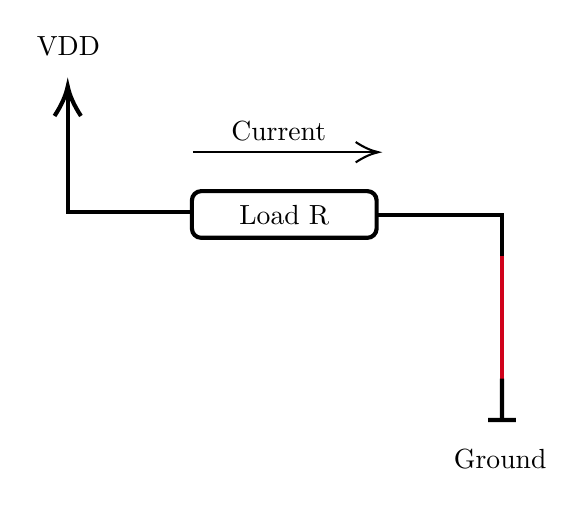
\begin{tikzpicture}[x=0.75pt,y=0.75pt,yscale=-1,xscale=1]
%uncomment if require: \path (0,240); %set diagram left start at 0, and has height of 240

%Straight Lines [id:da008984438739192413] 
\draw [color={rgb, 255:red, 0; green, 0; blue, 0 }  ,draw opacity=1 ][line width=1.5]    (91,99) -- (31.67,99) -- (31.67,41.33) ;
\draw [shift={(31.67,38.33)}, rotate = 450] [color={rgb, 255:red, 0; green, 0; blue, 0 }  ,draw opacity=1 ][line width=1.5]    (14.21,-6.37) .. controls (9.04,-2.99) and (4.3,-0.87) .. (0,0) .. controls (4.3,0.87) and (9.04,2.99) .. (14.21,6.37)   ;

%Rounded Rect [id:dp7662687261949606] 
\draw  [line width=1.5]  (91.5,93.25) .. controls (91.5,90.76) and (93.51,88.75) .. (96,88.75) -- (176,88.75) .. controls (178.49,88.75) and (180.5,90.76) .. (180.5,93.25) -- (180.5,106.75) .. controls (180.5,109.24) and (178.49,111.25) .. (176,111.25) -- (96,111.25) .. controls (93.51,111.25) and (91.5,109.24) .. (91.5,106.75) -- cycle ;
%Straight Lines [id:da19872085195301215] 
\draw [line width=1.5]    (181,100.25) -- (240.75,100.25) -- (240.75,120.13) ;


%Straight Lines [id:da8624965983535746] 
\draw [color={rgb, 255:red, 208; green, 2; blue, 27 }  ,draw opacity=1 ][line width=1.5]    (240.88,120.13) -- (240.88,179.13) ;


%Straight Lines [id:da9869704930235617] 
\draw [line width=1.5]    (240.88,179.13) -- (240.9,199) ;
\draw [shift={(240.9,199)}, rotate = 269.93] [color={rgb, 255:red, 0; green, 0; blue, 0 }  ][line width=1.5]    (0,6.71) -- (0,-6.71)   ;

%Straight Lines [id:da3727804380230437] 
\draw [line width=0.75]    (92,70) -- (179.33,70) ;
\draw [shift={(181.33,70)}, rotate = 180] [color={rgb, 255:red, 0; green, 0; blue, 0 }  ][line width=0.75]    (10.93,-4.9) .. controls (6.95,-2.3) and (3.31,-0.67) .. (0,0) .. controls (3.31,0.67) and (6.95,2.3) .. (10.93,4.9)   ;


% Text Node
\draw (136,100) node [scale=1] [align=left] {Load R};
% Text Node
\draw (133.33,59.67) node  [align=left] {Current};
% Text Node
\draw (240,218) node  [align=left] {Ground};
% Text Node
\draw (32,19) node  [align=left] {VDD};


\end{tikzpicture}
    \caption{short(low resistance) circuit between the load and the ground.} \label{fig:circuit1}
\end{figure}

If we connect an open circuit after the load (See Figure \ref{fig:circuit2}), it will increase the resistance to a very high value, causing the current to become zero effectively. If the current is zero then the voltage is also zero (Ohm's Law).

\begin{figure}[!ht]
    \centering
    

\tikzset{every picture/.style={line width=0.75pt}} %set default line width to 0.75pt        

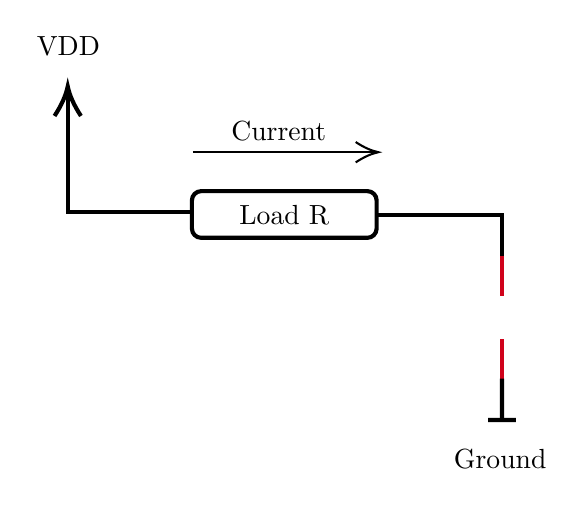
\begin{tikzpicture}[x=0.75pt,y=0.75pt,yscale=-1,xscale=1]
%uncomment if require: \path (0,240); %set diagram left start at 0, and has height of 240

%Straight Lines [id:da008984438739192413] 
\draw [color={rgb, 255:red, 0; green, 0; blue, 0 }  ,draw opacity=1 ][line width=1.5]    (91,99) -- (31.67,99) -- (31.67,41.33) ;
\draw [shift={(31.67,38.33)}, rotate = 450] [color={rgb, 255:red, 0; green, 0; blue, 0 }  ,draw opacity=1 ][line width=1.5]    (14.21,-6.37) .. controls (9.04,-2.99) and (4.3,-0.87) .. (0,0) .. controls (4.3,0.87) and (9.04,2.99) .. (14.21,6.37)   ;

%Rounded Rect [id:dp7662687261949606] 
\draw  [line width=1.5]  (91.5,93.25) .. controls (91.5,90.76) and (93.51,88.75) .. (96,88.75) -- (176,88.75) .. controls (178.49,88.75) and (180.5,90.76) .. (180.5,93.25) -- (180.5,106.75) .. controls (180.5,109.24) and (178.49,111.25) .. (176,111.25) -- (96,111.25) .. controls (93.51,111.25) and (91.5,109.24) .. (91.5,106.75) -- cycle ;
%Straight Lines [id:da19872085195301215] 
\draw [line width=1.5]    (181,100.25) -- (240.75,100.25) -- (240.75,120.13) ;


%Straight Lines [id:da8624965983535746] 
\draw [color={rgb, 255:red, 208; green, 2; blue, 27 }  ,draw opacity=1 ][line width=1.5]    (240.88,160) -- (240.88,179.13) ;


%Straight Lines [id:da9869704930235617] 
\draw [line width=1.5]    (240.88,179.13) -- (240.9,199) ;
\draw [shift={(240.9,199)}, rotate = 269.93] [color={rgb, 255:red, 0; green, 0; blue, 0 }  ][line width=1.5]    (0,6.71) -- (0,-6.71)   ;

%Straight Lines [id:da3727804380230437] 
\draw [line width=0.75]    (92,70) -- (179.33,70) ;
\draw [shift={(181.33,70)}, rotate = 180] [color={rgb, 255:red, 0; green, 0; blue, 0 }  ][line width=0.75]    (10.93,-4.9) .. controls (6.95,-2.3) and (3.31,-0.67) .. (0,0) .. controls (3.31,0.67) and (6.95,2.3) .. (10.93,4.9)   ;

%Straight Lines [id:da775249144810833] 
\draw [color={rgb, 255:red, 208; green, 2; blue, 27 }  ,draw opacity=1 ][line width=1.5]    (240.75,120.13) -- (240.75,139.25) ;



% Text Node
\draw (136,100) node [scale=1] [align=left] {Load R};
% Text Node
\draw (133.33,59.67) node  [align=left] {Current};
% Text Node
\draw (240,218) node  [align=left] {Ground};
% Text Node
\draw (32,19) node  [align=left] {VDD};


\end{tikzpicture}

    \caption{open circuit after the load.} \label{fig:circuit2}
\end{figure}

\subsubsection{Connecting in parallel}

If we connect an open circuit in parallel to the load (See Figure \ref{fig:circuit3}), the current will flow only through the load path, so the current on the open circuit will be 0. However, the voltage drop between both points of the open circuit will be the same as the drop between the load sides.

\begin{figure}[!ht]
    \centering
    

\tikzset{every picture/.style={line width=0.75pt}} %set default line width to 0.75pt        

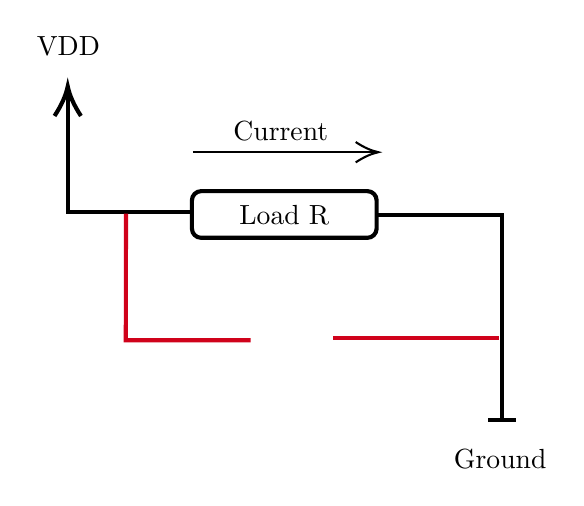
\begin{tikzpicture}[x=0.75pt,y=0.75pt,yscale=-1,xscale=1]
%uncomment if require: \path (0,250); %set diagram left start at 0, and has height of 250

%Straight Lines [id:da008984438739192413] 
\draw [color={rgb, 255:red, 0; green, 0; blue, 0 }  ,draw opacity=1 ][line width=1.5]    (91,99) -- (31.67,99) -- (31.67,41.33) ;
\draw [shift={(31.67,38.33)}, rotate = 450] [color={rgb, 255:red, 0; green, 0; blue, 0 }  ,draw opacity=1 ][line width=1.5]    (14.21,-6.37) .. controls (9.04,-2.99) and (4.3,-0.87) .. (0,0) .. controls (4.3,0.87) and (9.04,2.99) .. (14.21,6.37)   ;

%Rounded Rect [id:dp7662687261949606] 
\draw  [line width=1.5]  (91.5,93.25) .. controls (91.5,90.76) and (93.51,88.75) .. (96,88.75) -- (176,88.75) .. controls (178.49,88.75) and (180.5,90.76) .. (180.5,93.25) -- (180.5,106.75) .. controls (180.5,109.24) and (178.49,111.25) .. (176,111.25) -- (96,111.25) .. controls (93.51,111.25) and (91.5,109.24) .. (91.5,106.75) -- cycle ;
%Straight Lines [id:da19872085195301215] 
\draw [line width=1.5]    (181,100.25) -- (240.75,100.25) -- (240.75,199) ;
\draw [shift={(240.75,199)}, rotate = 270] [color={rgb, 255:red, 0; green, 0; blue, 0 }  ][line width=1.5]    (0,6.71) -- (0,-6.71)   ;

%Straight Lines [id:da3727804380230437] 
\draw [line width=0.75]    (92,70) -- (179.33,70) ;
\draw [shift={(181.33,70)}, rotate = 180] [color={rgb, 255:red, 0; green, 0; blue, 0 }  ][line width=0.75]    (10.93,-4.9) .. controls (6.95,-2.3) and (3.31,-0.67) .. (0,0) .. controls (3.31,0.67) and (6.95,2.3) .. (10.93,4.9)   ;

%Straight Lines [id:da4889722354710415] 
\draw [color={rgb, 255:red, 208; green, 2; blue, 27 }  ,draw opacity=1 ][line width=1.5]    (59.73,99.6) -- (59.65,160.6) -- (119.75,160.6) ;


%Straight Lines [id:da969741666977372] 
\draw [color={rgb, 255:red, 208; green, 2; blue, 27 }  ,draw opacity=1 ][line width=1.5]    (159.5,159.67) -- (239.25,159.67) ;



% Text Node
\draw (136,100) node [scale=1] [align=left] {Load R};
% Text Node
\draw (134.33,59.67) node  [align=left] {Current};
% Text Node
\draw (240,218) node  [align=left] {Ground};
% Text Node
\draw (32,19) node  [align=left] {VDD};


\end{tikzpicture}
    \caption{A close circuit in parallel to the load.} \label{fig:circuit3}
\end{figure}

If we connect a short circuit in parallel to the load (See Figure \ref{fig:circuit4}), the current will ``prefer" flowing through it rather than through the load, so the current through the load will be equal to zero, while the current through the short circuit will be very high - by Ohm's law.

\begin{figure}[!ht]
    \centering
    

\tikzset{every picture/.style={line width=0.75pt}} %set default line width to 0.75pt        

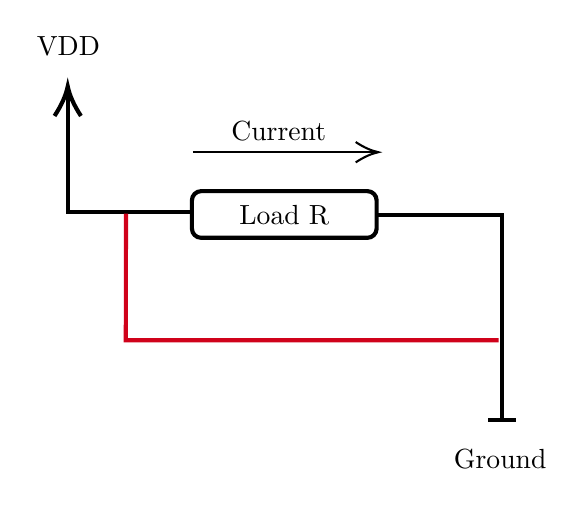
\begin{tikzpicture}[x=0.75pt,y=0.75pt,yscale=-1,xscale=1]
%uncomment if require: \path (0,230.3333282470703); %set diagram left start at 0, and has height of 230.3333282470703

%Straight Lines [id:da008984438739192413] 
\draw [color={rgb, 255:red, 0; green, 0; blue, 0 }  ,draw opacity=1 ][line width=1.5]    (91,99) -- (31.67,99) -- (31.67,41.33) ;
\draw [shift={(31.67,38.33)}, rotate = 450] [color={rgb, 255:red, 0; green, 0; blue, 0 }  ,draw opacity=1 ][line width=1.5]    (14.21,-6.37) .. controls (9.04,-2.99) and (4.3,-0.87) .. (0,0) .. controls (4.3,0.87) and (9.04,2.99) .. (14.21,6.37)   ;

%Rounded Rect [id:dp7662687261949606] 
\draw  [line width=1.5]  (91.5,93.25) .. controls (91.5,90.76) and (93.51,88.75) .. (96,88.75) -- (176,88.75) .. controls (178.49,88.75) and (180.5,90.76) .. (180.5,93.25) -- (180.5,106.75) .. controls (180.5,109.24) and (178.49,111.25) .. (176,111.25) -- (96,111.25) .. controls (93.51,111.25) and (91.5,109.24) .. (91.5,106.75) -- cycle ;
%Straight Lines [id:da19872085195301215] 
\draw [line width=1.5]    (181,100.25) -- (240.75,100.25) -- (240.75,199) ;
\draw [shift={(240.75,199)}, rotate = 270] [color={rgb, 255:red, 0; green, 0; blue, 0 }  ][line width=1.5]    (0,6.71) -- (0,-6.71)   ;

%Straight Lines [id:da3727804380230437] 
\draw [line width=0.75]    (92,70) -- (179.33,70) ;
\draw [shift={(181.33,70)}, rotate = 180] [color={rgb, 255:red, 0; green, 0; blue, 0 }  ][line width=0.75]    (10.93,-4.9) .. controls (6.95,-2.3) and (3.31,-0.67) .. (0,0) .. controls (3.31,0.67) and (6.95,2.3) .. (10.93,4.9)   ;

%Straight Lines [id:da4889722354710415] 
\draw [color={rgb, 255:red, 208; green, 2; blue, 27 }  ,draw opacity=1 ][line width=1.5]    (59.73,99.6) -- (59.65,160.6) -- (239.33,160.6) ;



% Text Node
\draw (136,100) node [scale=1] [align=left] {Load R};
% Text Node
\draw (133.33,59.67) node  [align=left] {Current};
% Text Node
\draw (240,218) node  [align=left] {Ground};
% Text Node
\draw (32,19) node  [align=left] {VDD};


\end{tikzpicture}
    \caption{A short circuit in parallel to the load.} \label{fig:circuit4}
\end{figure}

Since the cable is not a perfect conductor, some of the energy will be consumes in the form of thermal work, so the cable will heat, and possibly melt and start a fire.

\section{Measuring Power Consumption}

Next, as an attackers, we want to measure the power consumption of this load, and to do so, we are going to use Ampermeter device.

\subsection{Ampermeter}

An Ampermeter (from \textbf{Am}pere \textbf{Meter}) is a device capable of measuring the amount of electric current going through it. It has very low resistance, so it doesn't interrupt the system connected to it.

\begin{figure}[!ht]
    \centering
    

\tikzset{every picture/.style={line width=0.75pt}} %set default line width to 0.75pt        

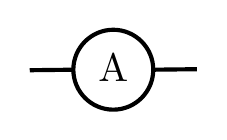
\begin{tikzpicture}[x=0.75pt,y=0.75pt,yscale=-1,xscale=1]
%uncomment if require: \path (0,80.33332824707031); %set diagram left start at 0, and has height of 80.33332824707031

%Shape: Circle [id:dp8443143357842926] 
\draw  [line width=1.5]  (42,40.58) .. controls (42,29.95) and (50.62,21.33) .. (61.25,21.33) .. controls (71.88,21.33) and (80.5,29.95) .. (80.5,40.58) .. controls (80.5,51.21) and (71.88,59.83) .. (61.25,59.83) .. controls (50.62,59.83) and (42,51.21) .. (42,40.58) -- cycle ;
%Straight Lines [id:da8989689187935987] 
\draw [line width=1.5]    (80.5,40.58) -- (101.5,40.33) ;


%Straight Lines [id:da08094666094700531] 
\draw [line width=1.5]    (21,40.83) -- (42,40.58) ;



% Text Node
\draw (61.25,39.58) node [scale=1.44] [align=left] {A};


\end{tikzpicture}
    \caption{Ampermeter Symbol in Circuit Diagrams.} \label{fig:ampermeter}
\end{figure}

\subsubsection{Using Ampermeter to measure power consumption}

We need to ``cut" the wire connected to the load and connect both sides to the Ampermeter.(See \Cref{fig:circuit5})

Doing so will cause all current flowing through the load to pass through the Ampermeter as well, so we will be able to read the current at any given time. The resistance of the Ampermeter is very low so it will not affect the voltage that going through the load that will have the same voltage drop as before. 

\begin{figure}[!ht]
    \centering
    

\tikzset{every picture/.style={line width=0.75pt}} %set default line width to 0.75pt        

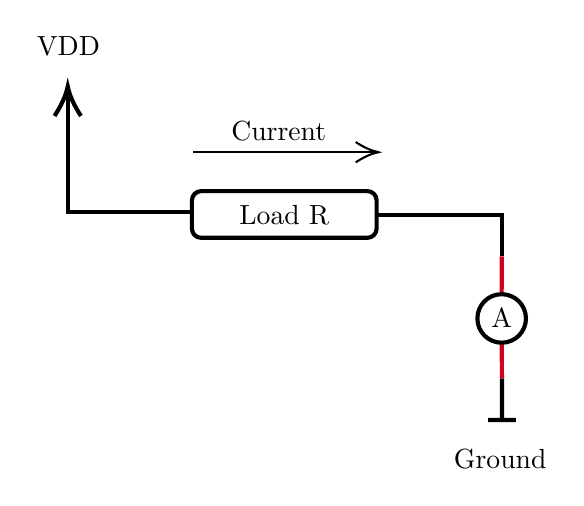
\begin{tikzpicture}[x=0.75pt,y=0.75pt,yscale=-1,xscale=1]
%uncomment if require: \path (0,240); %set diagram left start at 0, and has height of 240

%Straight Lines [id:da008984438739192413] 
\draw [color={rgb, 255:red, 0; green, 0; blue, 0 }  ,draw opacity=1 ][line width=1.5]    (91,99) -- (31.67,99) -- (31.67,41.33) ;
\draw [shift={(31.67,38.33)}, rotate = 450] [color={rgb, 255:red, 0; green, 0; blue, 0 }  ,draw opacity=1 ][line width=1.5]    (14.21,-6.37) .. controls (9.04,-2.99) and (4.3,-0.87) .. (0,0) .. controls (4.3,0.87) and (9.04,2.99) .. (14.21,6.37)   ;

%Rounded Rect [id:dp7662687261949606] 
\draw  [line width=1.5]  (91.5,93.25) .. controls (91.5,90.76) and (93.51,88.75) .. (96,88.75) -- (176,88.75) .. controls (178.49,88.75) and (180.5,90.76) .. (180.5,93.25) -- (180.5,106.75) .. controls (180.5,109.24) and (178.49,111.25) .. (176,111.25) -- (96,111.25) .. controls (93.51,111.25) and (91.5,109.24) .. (91.5,106.75) -- cycle ;
%Straight Lines [id:da19872085195301215] 
\draw [line width=1.5]    (181,100.25) -- (240.75,100.25) -- (240.75,120.13) ;


%Straight Lines [id:da8624965983535746] 
\draw [color={rgb, 255:red, 208; green, 2; blue, 27 }  ,draw opacity=1 ][line width=1.5]    (240.74,161.79) -- (240.88,179.13) ;


%Straight Lines [id:da9869704930235617] 
\draw [line width=1.5]    (240.88,179.13) -- (240.9,199) ;
\draw [shift={(240.9,199)}, rotate = 269.93] [color={rgb, 255:red, 0; green, 0; blue, 0 }  ][line width=1.5]    (0,6.71) -- (0,-6.71)   ;

%Straight Lines [id:da3727804380230437] 
\draw [line width=0.75]    (92,70) -- (179.33,70) ;
\draw [shift={(181.33,70)}, rotate = 180] [color={rgb, 255:red, 0; green, 0; blue, 0 }  ][line width=0.75]    (10.93,-4.9) .. controls (6.95,-2.3) and (3.31,-0.67) .. (0,0) .. controls (3.31,0.67) and (6.95,2.3) .. (10.93,4.9)   ;

%Straight Lines [id:da775249144810833] 
\draw [color={rgb, 255:red, 208; green, 2; blue, 27 }  ,draw opacity=1 ][line width=1.5]    (240.75,120.13) -- (240.74,138.4) ;


%Shape: Circle [id:dp5127141465445768] 
\draw  [line width=1.5]  (229.04,150.09) .. controls (229.04,143.63) and (234.28,138.4) .. (240.74,138.4) .. controls (247.2,138.4) and (252.44,143.63) .. (252.44,150.09) .. controls (252.44,156.55) and (247.2,161.79) .. (240.74,161.79) .. controls (234.28,161.79) and (229.04,156.55) .. (229.04,150.09) -- cycle ;

% Text Node
\draw (136,100) node [scale=1] [align=left] {Load R};
% Text Node
\draw (133.33,59.67) node  [align=left] {Current};
% Text Node
\draw (240,218) node  [align=left] {Ground};
% Text Node
\draw (32,19) node  [align=left] {VDD};
% Text Node
\draw (240.74,150.09) node  [align=left] {A};


\end{tikzpicture}
    \caption{an Ampermeter connected in serial.} \label{fig:circuit5}
\end{figure}

Now we will measure the current going through the ampermeter and next we will convert the current in order to find the power consumption of the load.

In case we know the voltage (i.e. a 5V battery, a 220V power socket), we can compute the power consumption: $P=I*V$.

The problem: sometimes, we don't want (or simply can't) cut the circuit after the load in order to connect an Ampermeter, and this is a way that the architect of the device are trying to protect it. So, let's see if we can use the ampermeter without cutting anything, and let's connect it in parallel to the load. (See \Cref{fig:circuit6})

\begin{figure}[!ht]
    \centering
    

\tikzset{every picture/.style={line width=0.75pt}} %set default line width to 0.75pt        

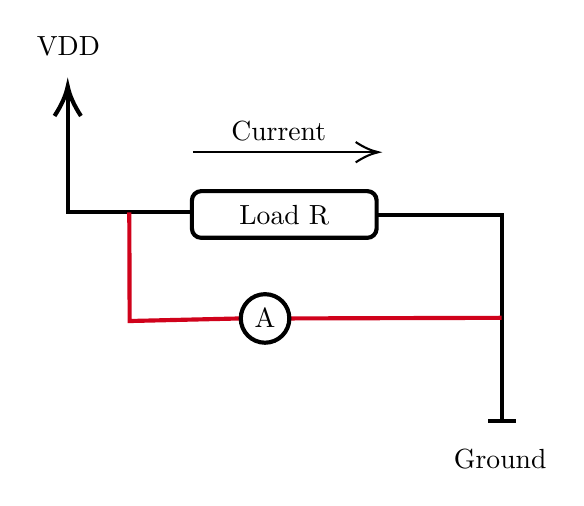
\begin{tikzpicture}[x=0.75pt,y=0.75pt,yscale=-1,xscale=1]
%uncomment if require: \path (0,240); %set diagram left start at 0, and has height of 240

%Straight Lines [id:da008984438739192413] 
\draw [color={rgb, 255:red, 0; green, 0; blue, 0 }  ,draw opacity=1 ][line width=1.5]    (91,99) -- (31.67,99) -- (31.67,41.33) ;
\draw [shift={(31.67,38.33)}, rotate = 450] [color={rgb, 255:red, 0; green, 0; blue, 0 }  ,draw opacity=1 ][line width=1.5]    (14.21,-6.37) .. controls (9.04,-2.99) and (4.3,-0.87) .. (0,0) .. controls (4.3,0.87) and (9.04,2.99) .. (14.21,6.37)   ;

%Rounded Rect [id:dp7662687261949606] 
\draw  [line width=1.5]  (91.5,93.25) .. controls (91.5,90.76) and (93.51,88.75) .. (96,88.75) -- (176,88.75) .. controls (178.49,88.75) and (180.5,90.76) .. (180.5,93.25) -- (180.5,106.75) .. controls (180.5,109.24) and (178.49,111.25) .. (176,111.25) -- (96,111.25) .. controls (93.51,111.25) and (91.5,109.24) .. (91.5,106.75) -- cycle ;
%Straight Lines [id:da19872085195301215] 
\draw [line width=1.5]    (181,100.25) -- (240.75,100.25) -- (240.75,199.33) ;
\draw [shift={(240.75,199.33)}, rotate = 270] [color={rgb, 255:red, 0; green, 0; blue, 0 }  ][line width=1.5]    (0,6.71) -- (0,-6.71)   ;

%Straight Lines [id:da8624965983535746] 
\draw [color={rgb, 255:red, 208; green, 2; blue, 27 }  ,draw opacity=1 ][line width=1.5]    (138.44,150.09) -- (240.75,149.79) ;


%Straight Lines [id:da3727804380230437] 
\draw [line width=0.75]    (92,70) -- (179.33,70) ;
\draw [shift={(181.33,70)}, rotate = 180] [color={rgb, 255:red, 0; green, 0; blue, 0 }  ][line width=0.75]    (10.93,-4.9) .. controls (6.95,-2.3) and (3.31,-0.67) .. (0,0) .. controls (3.31,0.67) and (6.95,2.3) .. (10.93,4.9)   ;

%Straight Lines [id:da775249144810833] 
\draw [color={rgb, 255:red, 208; green, 2; blue, 27 }  ,draw opacity=1 ][line width=1.5]    (61.33,99) -- (61.5,151.33) -- (115.04,150.09) ;


%Shape: Circle [id:dp5127141465445768] 
\draw  [line width=1.5]  (115.04,150.09) .. controls (115.04,143.63) and (120.28,138.4) .. (126.74,138.4) .. controls (133.2,138.4) and (138.44,143.63) .. (138.44,150.09) .. controls (138.44,156.55) and (133.2,161.79) .. (126.74,161.79) .. controls (120.28,161.79) and (115.04,156.55) .. (115.04,150.09) -- cycle ;

% Text Node
\draw (136,100) node [scale=1] [align=left] {Load R};
% Text Node
\draw (133.33,59.67) node  [align=left] {Current};
% Text Node
\draw (240,218) node  [align=left] {Ground};
% Text Node
\draw (32,19) node  [align=left] {VDD};
% Text Node
\draw (126.74,150.09) node  [align=left] {A};


\end{tikzpicture}
    \caption{An ampermeter connected in parallel to the load} \label{fig:circuit6}
\end{figure}

Connecting the ampermeter this way will burn the ampermeter as it has no resistance and so, all of the current will flow through it. So, instead of ampermeter we can use a voltmeter as follows (See \Cref{fig:circuit7}):

\subsection{Voltmeter}

\begin{figure}[!ht]
    \centering
    

\tikzset{every picture/.style={line width=0.75pt}} %set default line width to 0.75pt        

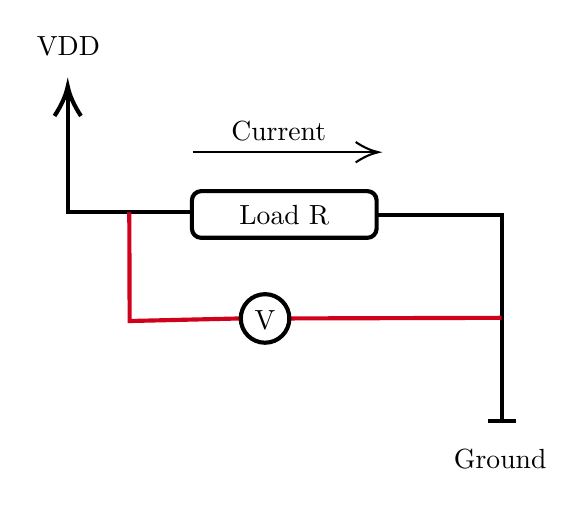
\begin{tikzpicture}[x=0.75pt,y=0.75pt,yscale=-1,xscale=1]
%uncomment if require: \path (0,240); %set diagram left start at 0, and has height of 240

%Straight Lines [id:da008984438739192413] 
\draw [color={rgb, 255:red, 0; green, 0; blue, 0 }  ,draw opacity=1 ][line width=1.5]    (91,99) -- (31.67,99) -- (31.67,41.33) ;
\draw [shift={(31.67,38.33)}, rotate = 450] [color={rgb, 255:red, 0; green, 0; blue, 0 }  ,draw opacity=1 ][line width=1.5]    (14.21,-6.37) .. controls (9.04,-2.99) and (4.3,-0.87) .. (0,0) .. controls (4.3,0.87) and (9.04,2.99) .. (14.21,6.37)   ;

%Rounded Rect [id:dp7662687261949606] 
\draw  [line width=1.5]  (91.5,93.25) .. controls (91.5,90.76) and (93.51,88.75) .. (96,88.75) -- (176,88.75) .. controls (178.49,88.75) and (180.5,90.76) .. (180.5,93.25) -- (180.5,106.75) .. controls (180.5,109.24) and (178.49,111.25) .. (176,111.25) -- (96,111.25) .. controls (93.51,111.25) and (91.5,109.24) .. (91.5,106.75) -- cycle ;
%Straight Lines [id:da19872085195301215] 
\draw [line width=1.5]    (181,100.25) -- (240.75,100.25) -- (240.75,199.33) ;
\draw [shift={(240.75,199.33)}, rotate = 270] [color={rgb, 255:red, 0; green, 0; blue, 0 }  ][line width=1.5]    (0,6.71) -- (0,-6.71)   ;

%Straight Lines [id:da8624965983535746] 
\draw [color={rgb, 255:red, 208; green, 2; blue, 27 }  ,draw opacity=1 ][line width=1.5]    (138.44,150.09) -- (240.75,149.79) ;


%Straight Lines [id:da3727804380230437] 
\draw [line width=0.75]    (92,70) -- (179.33,70) ;
\draw [shift={(181.33,70)}, rotate = 180] [color={rgb, 255:red, 0; green, 0; blue, 0 }  ][line width=0.75]    (10.93,-4.9) .. controls (6.95,-2.3) and (3.31,-0.67) .. (0,0) .. controls (3.31,0.67) and (6.95,2.3) .. (10.93,4.9)   ;

%Straight Lines [id:da775249144810833] 
\draw [color={rgb, 255:red, 208; green, 2; blue, 27 }  ,draw opacity=1 ][line width=1.5]    (61.33,99) -- (61.5,151.33) -- (115.04,150.09) ;


%Shape: Circle [id:dp5127141465445768] 
\draw  [line width=1.5]  (115.04,150.09) .. controls (115.04,143.63) and (120.28,138.4) .. (126.74,138.4) .. controls (133.2,138.4) and (138.44,143.63) .. (138.44,150.09) .. controls (138.44,156.55) and (133.2,161.79) .. (126.74,161.79) .. controls (120.28,161.79) and (115.04,156.55) .. (115.04,150.09) -- cycle ;

% Text Node
\draw (136,100) node [scale=1] [align=left] {Load R};
% Text Node
\draw (133.33,59.67) node  [align=left] {Current};
% Text Node
\draw (240,218) node  [align=left] {Ground};
% Text Node
\draw (32,19) node  [align=left] {VDD};
% Text Node
\draw (126.74,151.09) node  [align=left] {V};


\end{tikzpicture}
    \caption{a voltmeter connected in parallel to the load} \label{fig:circuit7}
\end{figure}

The voltmeter resistance is very very high so the current will not go through it. The voltmeter is measuring the voltage drop between one side of the load and the other side of it. If we want to measure the current using the voltmeter we are taking a load with a very small resistance and connect it as follows (See \Cref{fig:circuit8}):

\begin{figure}[!ht]
    \centering
    

\tikzset{every picture/.style={line width=0.75pt}} %set default line width to 0.75pt        

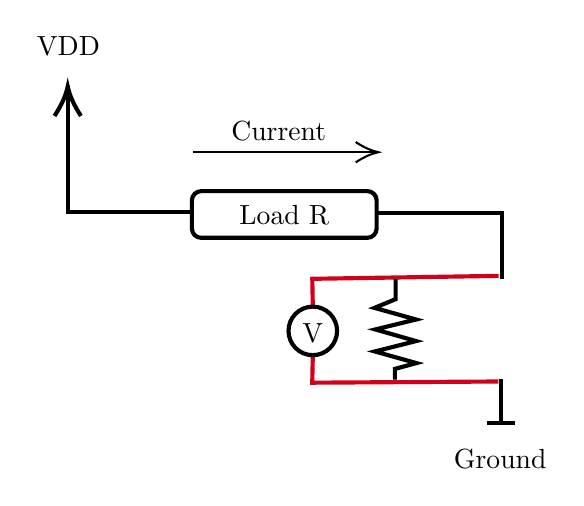
\begin{tikzpicture}[x=0.75pt,y=0.75pt,yscale=-1,xscale=1]
%uncomment if require: \path (0,230.3333282470703); %set diagram left start at 0, and has height of 230.3333282470703

%Straight Lines [id:da008984438739192413] 
\draw [color={rgb, 255:red, 0; green, 0; blue, 0 }  ,draw opacity=1 ][line width=1.5]    (91,99) -- (31.67,99) -- (31.67,41.33) ;
\draw [shift={(31.67,38.33)}, rotate = 450] [color={rgb, 255:red, 0; green, 0; blue, 0 }  ,draw opacity=1 ][line width=1.5]    (14.21,-6.37) .. controls (9.04,-2.99) and (4.3,-0.87) .. (0,0) .. controls (4.3,0.87) and (9.04,2.99) .. (14.21,6.37)   ;

%Rounded Rect [id:dp7662687261949606] 
\draw  [line width=1.5]  (91.5,93.25) .. controls (91.5,90.76) and (93.51,88.75) .. (96,88.75) -- (176,88.75) .. controls (178.49,88.75) and (180.5,90.76) .. (180.5,93.25) -- (180.5,106.75) .. controls (180.5,109.24) and (178.49,111.25) .. (176,111.25) -- (96,111.25) .. controls (93.51,111.25) and (91.5,109.24) .. (91.5,106.75) -- cycle ;
%Straight Lines [id:da19872085195301215] 
\draw [line width=1.5]    (181,99.25) -- (240.75,99.25) -- (240.75,131.08) ;


%Straight Lines [id:da8624965983535746] 
\draw [color={rgb, 255:red, 208; green, 2; blue, 27 }  ,draw opacity=1 ][line width=1.5]    (149.74,144.4) -- (149.5,131) -- (239.25,129.58) ;


%Straight Lines [id:da3727804380230437] 
\draw [line width=0.75]    (92,70) -- (179.33,70) ;
\draw [shift={(181.33,70)}, rotate = 180] [color={rgb, 255:red, 0; green, 0; blue, 0 }  ][line width=0.75]    (10.93,-4.9) .. controls (6.95,-2.3) and (3.31,-0.67) .. (0,0) .. controls (3.31,0.67) and (6.95,2.3) .. (10.93,4.9)   ;

%Straight Lines [id:da775249144810833] 
\draw [color={rgb, 255:red, 208; green, 2; blue, 27 }  ,draw opacity=1 ][line width=1.5]    (149.74,167.79) -- (149.48,181.05) -- (239.19,180.47) ;


%Shape: Circle [id:dp5127141465445768] 
\draw  [line width=1.5]  (138.04,156.09) .. controls (138.04,149.63) and (143.28,144.4) .. (149.74,144.4) .. controls (156.2,144.4) and (161.44,149.63) .. (161.44,156.09) .. controls (161.44,162.55) and (156.2,167.79) .. (149.74,167.79) .. controls (143.28,167.79) and (138.04,162.55) .. (138.04,156.09) -- cycle ;
%Straight Lines [id:da5151277448838241] 
\draw [line width=1.5]    (240.32,179.37) -- (240.32,200.37) ;
\draw [shift={(240.32,200.37)}, rotate = 270] [color={rgb, 255:red, 0; green, 0; blue, 0 }  ][line width=1.5]    (0,6.71) -- (0,-6.71)   ;

%Straight Lines [id:da45585704731206445] 
\draw [line width=1.5]    (189.67,131.2) -- (189.67,140.8) -- (179.47,145) -- (199.47,150.6) -- (179.87,155.4) -- (199.47,161) -- (179.67,166) -- (199.67,171.6) -- (189.27,174.4) -- (189.27,179.6) ;



% Text Node
\draw (136,100) node [scale=1] [align=left] {Load R};
% Text Node
\draw (133.33,59.67) node  [align=left] {Current};
% Text Node
\draw (240,218) node  [align=left] {Ground};
% Text Node
\draw (32,19) node  [align=left] {VDD};
% Text Node
\draw (149.74,157.09) node  [align=left] {V};


\end{tikzpicture}
    \caption{Circuit 8.} \label{fig:circuit8}
\end{figure}

This way, because of the current divider, by connecting a Voltmeter in parallel with a very small and accurate resistor, we can measure the electric current using Ohm's law: $I=V/R$
 
Summary: we learned what is Power Consumption and how we can measure it.
A very important fact is that \textbf{Power Consumption varies with time!}.
If we can find a relationship between the secret information we want to extract and the power consumption, we can recover this information by measuring the power consumption over time.

\subsection{Types of electronic components}

In general there are two types of elements in the circuit, the first one are Passive devices like a resistors (a passive two-terminal electrical component that implements electrical resistance as a circuit element), inductors (is a passive two-terminal electrical component that stores energy in a magnetic field when electric current flows through it), capacitors and diodes. And there are Active devices like transistors (a semiconductor device used to amplify or switch electronic signals and electrical power), amplifiers (an electronic device that can increase the power of a signal (a time-varying voltage or current)) and ICs. From our perspective, the Active devices are much more interesting for us (attackers) as they are using electricity in order to control electricity. One example can be an amplifier that has audio signal and power supply as inputs and it generates a greater audio signal as an output using the power supply. 

Another interesting active element for this course is a transistor. In an integrated circuits, there are a lot of active devices such as transistors  that if we can analyze their behavior we can learn about the data that they are processing. So when we look at the final consumption of these active elements, we can figure out some kind of secrets.

There are many kind of transistors and we will concentrate on understanding a certain type called Field-Effect Transistor.

\begin{figure}[!ht]
	\centering
	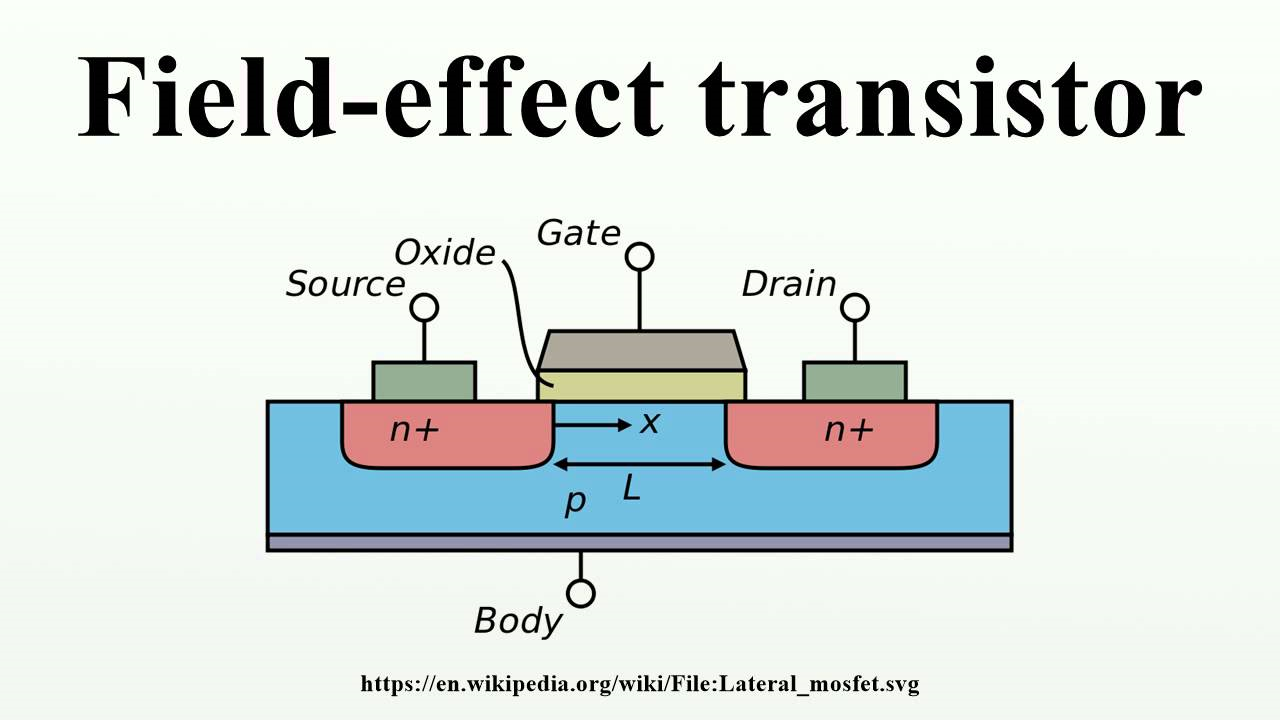
\includegraphics{images/field_effect_transistor.png}
	\caption{Field-Effect Transistor.} \label{fig:field_effect_transistor}
\end{figure}

\subsection{Field-Effect Transistor}

The field-effect transistor (FET) is an electronic device which uses an electric field to control the flow of current. FETs are 3-terminalled devices, having a source, gate, and drain terminal. FETs control the flow of current by the application of a voltage to the gate terminal, which in turn alters the conductivity between the drain and source terminals. In order to understand FET first we need to dive into the basics of semiconductors.

\subsection{Semiconductors}

A semiconductor is a substance, usually a solid chemical element or compound, that can conduct electricity under some conditions but not others, making it a good medium for the control of electrical current. Its conductance varies depending on the current or voltage applied to a control electrode, or on the intensity of irradiation by infrared (IR), visible light, ultraviolet (UV), or X rays. In general, transistors are made of semiconducting materials such as silicon. There are a conductor like copper or gold and there are insulators like plastic or glass.

Silicon atom has three parts: neutrons (not relevant for our use), protons with the positive charge (heavy) and electrons that have the negative charge and they are small and dynamic. Silicon atom has four electrons in its outer orbital and when we have a crystal silicon those 4 electrons are set in place very nicely. It means that pure silicon is a very bad conductor as  conducting means that the electrons can move around and in this case they are very comfortable where they are.

Metals can be good conductors of electricity as they have ``free electrons" that can move easily from atom to atom, the electricity involves the flow of electrons. As all of the outer electrons in Silicon crystal are involved in perfect covalent bonds, they cannot move around. So, silicon crystal is nearly insulator and very little electricity will flow through it. We can change the behavior of  the silicon and turn it into a conductor by doping it. In doping, we mix a small amount of an impurity into the silicon crystal.

There are two types of impurities:
\begin{itemize}
    \item N-type – where phosphorus or arsenic is added to the silicon in small quantities. They both have  five outer electrons, so one of them is out of place when they get into the silicon lattice. While having nothing to bond to, the fifth electron is free to move around. As electrons have a negative charge, this kind of impurity called N-type.
    \item P-type - where boron or gallium is added to the silicon. They both have only three outer electrons. So, when we mixed them into the silicon lattice, there will be ``holes" in the lattice where a silicon electron has nothing to bond to. The hole is looking for an electron from a neighbor atom and when that's happens the hole is ``moving". As the absence of an electron creates the effect of a positive charge, this kind of impurity called P-type.
\end{itemize}

\subsection{ How does Field-Effect Transistor work? }

In the Field-Effect Transistor there are (as shown in \Cref{fig:field_effect_transistor}) n+ areas (N-type) and P area (P-type). The n+ area contains a lot of free electrons and the P area contains a lot of 'holes'. When no electricity is connected to the gate, the free electrons from the N+ are moving to the holes so there are no free electrons within the semiconductor itself. That means electrons can't move from the source to the drain i.e. open circuit. When electricity is connected to the gate it charge a lot of free electrons to it. The free electrons in the gate can't move to the silicon itself as there is an oxide layer between them, but is pushes the electrons in the silicon down to the body in a way there are holes between the source and the drain. That way electrons can move from the source to the drain freely and we have close circuit. 

\begin{figure}[!ht]
    \centering
    

\tikzset{every picture/.style={line width=0.75pt}} %set default line width to 0.75pt        

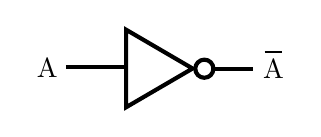
\begin{tikzpicture}[x=0.75pt,y=0.75pt,yscale=-1,xscale=1]
%uncomment if require: \path (0,219); %set diagram left start at 0, and has height of 219

%Straight Lines [id:da07885295239893186] 
\draw [line width=1.5]    (40,39.33) -- (68.5,39.33) ;


%Straight Lines [id:da2596764371394711] 
\draw [line width=1.5]    (110.02,40.17) -- (130.25,40.17) ;

\draw [shift={(106.67,40.17)}, rotate = 0] [color={rgb, 255:red, 0; green, 0; blue, 0 }  ][line width=1.5]      (0, 0) circle [x radius= 4.36, y radius= 4.36]   ;
%Straight Lines [id:da4451475450468101] 
\draw [line width=0.75]    (135.67,32.17) -- (144,32.17) ;


%Flowchart: Extract [id:dp4235554887602122] 
\draw  [line width=1.5]  (101,40.07) -- (69,58.73) -- (69,21.4) -- cycle ;

% Text Node
\draw (31,40) node  [align=left] {A};
% Text Node
\draw (140,40.5) node  [align=left] {A};


\end{tikzpicture}
    \caption{NOT Gate.} \label{fig:not}
\end{figure}

\subsection{ NOT Gate CMOS}

\begin{figure}[!ht]
    \centering
    

\tikzset{every picture/.style={line width=0.75pt}} %set default line width to 0.75pt        

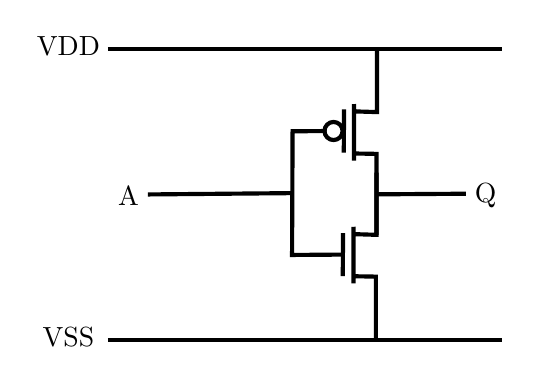
\begin{tikzpicture}[x=0.75pt,y=0.75pt,yscale=-1,xscale=1]
%uncomment if require: \path (0,201.3333282470703); %set diagram left start at 0, and has height of 201.3333282470703

%Straight Lines [id:da07885295239893186] 
\draw [line width=1.5]    (51,30.33) -- (240.75,30.33) ;


%Straight Lines [id:da39856222237487815] 
\draw [line width=1.5]    (180.67,30.67) -- (180.67,60.67) -- (169.71,60.33) -- (169.6,56.8) -- (169.6,84.05) -- (169.6,80.62) -- (180.4,80.8) -- (180.4,119.81) ;


%Straight Lines [id:da5857134524935192] 
\draw [line width=1.5]    (180.4,89.81) -- (180.4,119.81) -- (169.45,119.47) -- (169.33,115.94) -- (169.33,143.19) -- (169.33,139.76) -- (180.13,139.94) -- (180.13,170) ;


%Straight Lines [id:da21313521807196745] 
\draw [line width=1.5]    (51,170.33) -- (240.75,170.33) ;


%Straight Lines [id:da5667092258145612] 
\draw [line width=1.5]    (180.4,100.3) -- (223.5,100) ;


%Straight Lines [id:da6991442899200719] 
\draw [line width=1.5]    (164.67,80.16) -- (164.8,59.4) ;


%Straight Lines [id:da08031166754703278] 
\draw [line width=1.5]    (164.25,129.33) -- (139.75,129.5) -- (140,69.92) -- (156.38,69.8) ;
\draw [shift={(159.73,69.78)}, rotate = 359.6] [color={rgb, 255:red, 0; green, 0; blue, 0 }  ][line width=1.5]      (0, 0) circle [x radius= 4.36, y radius= 4.36]   ;

%Straight Lines [id:da21308267181792218] 
\draw [line width=1.5]    (164.18,139.71) -- (164.32,118.96) ;


%Straight Lines [id:da40299410186396645] 
\draw [line width=1.5]    (70.25,100.35) -- (139.88,99.71) ;



% Text Node
\draw (32,29) node  [align=left] {VDD};
% Text Node
\draw (32,169) node  [align=left] {VSS};
% Text Node
\draw (233,101) node  [align=left] {Q};
% Text Node
\draw (61,101) node  [align=left] {A};


\end{tikzpicture}
    \caption{Circuit 9.} \label{fig:circuit9}
\end{figure}

How does CMOS work? When the voltage of input A is low A = 0, the upper transistor's channel is closed and we have a connection between Vdd(1) and Q, so Q = 1, this is a Pull Up Network. And when the voltage of input A is high, then the lower transistor's channel is closed and we have a connection between Vss(0) and Q, so Q = 0, this is a Pull Down Network. A question is raised – when does this circuit consume power? There is almost no power consume as there is no connection between Vdd and Vss at any time. Although when CMOS is switching between states, there is a minor power usage and we will see how we can use it for our purpose.

Following is the NOT table:

\begin{table}
    \centering
    \caption{NOT gate truth table.}
    \begin{tabular}{llll}
        \toprule
        \textbf{input}  & A     & 0 & 1 \\ \midrule
        \textbf{output} & Not A & 1 & 0 \\ \bottomrule
    \end{tabular}
\end{table} 

\subsection{ AND Gate CMOS}

Next we will see how to build a bit more complicated gate using 4 transistors. Following is the AND gate diagram:

\begin{figure}[!ht]
    \centering
    

\tikzset{every picture/.style={line width=0.75pt}} %set default line width to 0.75pt        

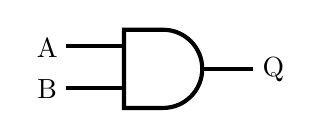
\begin{tikzpicture}[x=0.75pt,y=0.75pt,yscale=-1,xscale=1]
%uncomment if require: \path (0,80.33332824707031); %set diagram left start at 0, and has height of 80.33332824707031

%Straight Lines [id:da07885295239893186] 
\draw [line width=1.5]    (40,29.33) -- (68.5,29.33) ;


%Flowchart: Delay [id:dp4724078764954891] 
\draw  [line width=1.5]  (68,21.33) -- (86.83,21.33) .. controls (97.23,21.33) and (105.67,29.77) .. (105.67,40.17) .. controls (105.67,50.57) and (97.23,59) .. (86.83,59) -- (68,59) -- cycle ;
%Straight Lines [id:da5877789079181] 
\draw [line width=1.5]    (40,49.33) -- (68.5,49.33) ;


%Straight Lines [id:da2596764371394711] 
\draw [line width=1.5]    (106.67,40.17) -- (130.25,40.17) ;



% Text Node
\draw (31,30) node  [align=left] {A};
% Text Node
\draw (31,50) node  [align=left] {B};
% Text Node
\draw (140,40.5) node  [align=left] {Q};


\end{tikzpicture}
    \caption{AND Gate.} \label{fig:and}
\end{figure}

We will implement the gate using 4 transistors to support the following AND table:

\begin{table}[!ht]
    \centering
    \caption{AND gate truth table.}
    \begin{tabular}{lllll}
        \toprule
        \textbf{input a} & 0 & 0 & 1 & 1 \\ \midrule
        \textbf{input b} & 0 & 1 & 0 & 1 \\ \midrule
        \textbf{output}  & 0 & 0 & 0 & 1 \\ \bottomrule
    \end{tabular}
\end{table}

First we want to build the Pull Up Network, so for input A and B, for A=B=1 then the output Q is 1.
Then we will build the Pull Down Network to support the other combination from the table to deliver 0 as the output Q. Sometimes we don't want to have combination using the circuits, but we want to store information in it, next we will talk about another type of circuits called storage circuit or Sequential Circuit.

\subsection{ Storage/Sequential Circuit }

A latch or flip-flop is a circuit that has two stable states and can be used to store state information. 
\begin{figure}[!ht]
    \centering
    

\tikzset{every picture/.style={line width=0.75pt}} %set default line width to 0.75pt        

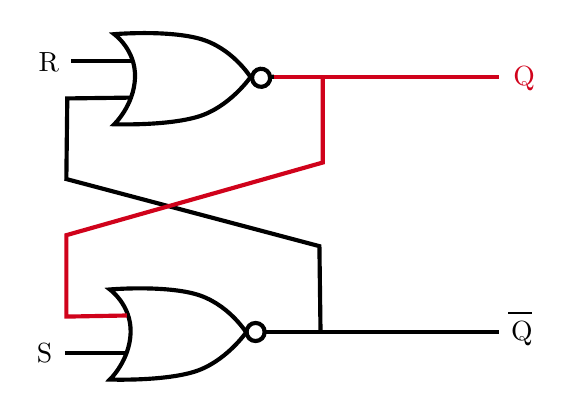
\begin{tikzpicture}[x=0.75pt,y=0.75pt,yscale=-1,xscale=1]
%uncomment if require: \path (0,210.66666412353516); %set diagram left start at 0, and has height of 210.66666412353516

%Shape: Polygon Curved [id:ds6291230594537647] 
\draw  [color={rgb, 255:red, 0; green, 0; blue, 0 }  ,draw opacity=1 ][line width=1.5]  (64.57,15.54) .. controls (64.57,15.54) and (75.02,23.03) .. (74.57,36.44) .. controls (74.11,49.84) and (64.57,58.93) .. (64.57,58.93) .. controls (64.57,58.93) and (89.67,59.83) .. (104.89,55.29) .. controls (120.12,50.74) and (130.23,36.21) .. (130.23,36.21) .. controls (130.23,36.21) and (121.33,21.89) .. (105.43,17.64) .. controls (89.52,13.4) and (64.57,15.54) .. (64.57,15.54) -- cycle ;
%Straight Lines [id:da32731251553352636] 
\draw [color={rgb, 255:red, 0; green, 0; blue, 0 }  ,draw opacity=1 ][line width=1.5]    (43.93,28.6) -- (72.96,28.6) ;


%Straight Lines [id:da3869103872130202] 
\draw [color={rgb, 255:red, 0; green, 0; blue, 0 }  ,draw opacity=1 ][line width=1.5]    (163.94,158.49) -- (163.41,117.67) -- (41.48,85.33) -- (41.94,46.49) -- (72.16,46.1) ;


%Straight Lines [id:da1720618143634285] 
\draw [color={rgb, 255:red, 0; green, 0; blue, 0 }  ,draw opacity=1 ][line width=1.5]    (138.66,36.27) -- (141.5,36.02) ;

\draw [shift={(135.32,36.55)}, rotate = 355.1] [color={rgb, 255:red, 0; green, 0; blue, 0 }  ,draw opacity=1 ][line width=1.5]      (0, 0) circle [x radius= 4.36, y radius= 4.36]   ;
%Straight Lines [id:da9259051839045029] 
\draw [color={rgb, 255:red, 0; green, 0; blue, 0 }  ,draw opacity=1 ][line width=1.5]    (136.02,159.02) -- (250,159.02) ;

\draw [shift={(132.67,159.02)}, rotate = 0] [color={rgb, 255:red, 0; green, 0; blue, 0 }  ,draw opacity=1 ][line width=1.5]      (0, 0) circle [x radius= 4.36, y radius= 4.36]   ;
%Shape: Polygon Curved [id:ds45090218745840094] 
\draw  [color={rgb, 255:red, 0; green, 0; blue, 0 }  ,draw opacity=1 ][line width=1.5]  (62.45,138.53) .. controls (62.45,138.53) and (72.9,146.03) .. (72.45,159.43) .. controls (71.99,172.84) and (62.45,181.93) .. (62.45,181.93) .. controls (62.45,181.93) and (87.55,182.82) .. (102.77,178.28) .. controls (118,173.74) and (128.11,159.21) .. (128.11,159.21) .. controls (128.11,159.21) and (119.21,144.88) .. (103.3,140.64) .. controls (87.4,136.4) and (62.45,138.53) .. (62.45,138.53) -- cycle ;
%Straight Lines [id:da4647074828700599] 
\draw [color={rgb, 255:red, 0; green, 0; blue, 0 }  ,draw opacity=1 ][line width=1.5]    (40.75,169.09) -- (69.78,169.09) ;


%Straight Lines [id:da5333172740033338] 
\draw [color={rgb, 255:red, 208; green, 2; blue, 27 }  ,draw opacity=1 ][line width=1.5]    (165,36.02) -- (165,77.38) -- (41.48,112.37) -- (41.48,151.6) -- (70.64,151.07) ;


%Straight Lines [id:da5430278461164106] 
\draw [color={rgb, 255:red, 208; green, 2; blue, 27 }  ,draw opacity=1 ][line width=1.5]    (141.5,36.02) -- (250,36.02) ;


%Straight Lines [id:da9737841576113742] 
\draw    (254.5,149.67) -- (266,149.67) ;



% Text Node
\draw (33,29) node  [align=left] {R};
% Text Node
\draw (31,169) node  [align=left] {S};
% Text Node
\draw (262,37) node  [align=left] {\textcolor[rgb]{0.82,0.01,0.11}{Q}};
% Text Node
\draw (261,160) node  [align=left] {Q};


\end{tikzpicture}
    \caption{Flipflop.} \label{fig:flipflop}
\end{figure}

The circuit can be made to change state by signals applied to one or more control inputs and will have one or two outputs. It is the basic storage element in sequential logic. Flip-flops and latches are fundamental building blocks of digital electronics systems used in computers, communications, and many other types of systems.

A flip-flop is a device which stores a single bit (binary digit) of data; one of its two states represents a ``one" and the other represents a ``zero". Such data storage can be used for storage of state, and such a circuit is described as sequential logic in electronics. When used in a finite-state machine, the output and next state depend not only on its current input, but also on its current state (and hence, previous inputs). It can also be used for counting of pulses, and for synchronizing variably-timed input signals to some reference timing signal.

Flip-flops can be either level-triggered (asynchronous, transparent or opaque) or edge-triggered (synchronous, or clocked). The term flip-flop has historically referred generically to both level-triggered and edge-triggered circuits that store a single bit of data using gates. We will refer Flip-Flop as edge-triggered i.e. clocked synchronized.

Flip-flop has to legs – data and clock, for each storage element in the circuit the data changes at the clock signal and so we have an amplified signal that we can monitor as attackers and try to learn the secret behind it.

 \subsection { Core I7 chip }
 
Following is the core I7 chip image:

\begin{figure}[!ht]
	\centering
	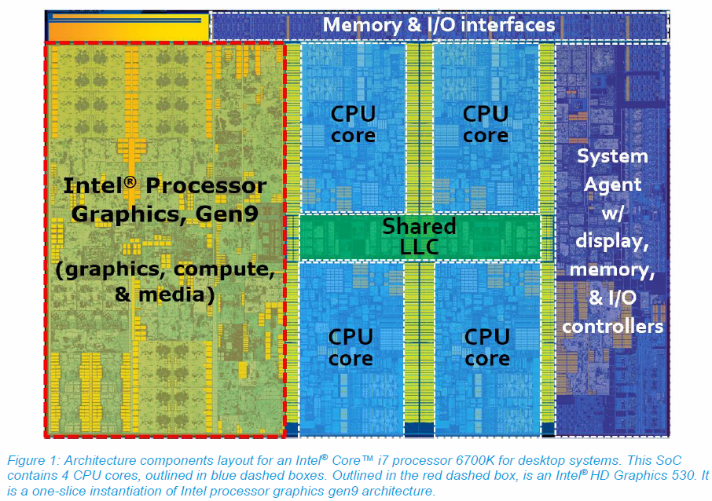
\includegraphics{images/i7.png}
	\caption{Intel i7.} \label{fig:i7}
\end{figure}

We can see ordered items that are the storage elements, there are 24 items that are the GPUs and they have a little memory next to the (upper left). The CPU core has also a cash memory in it.

\subsection { Power Consumption is Variable }

Next we will see how to get secrets from the power consumption.

\begin{figure}[!ht]
    \centering
    \tikzset{every picture/.style={line width=0.75pt}} %set default line width to 0.75pt        
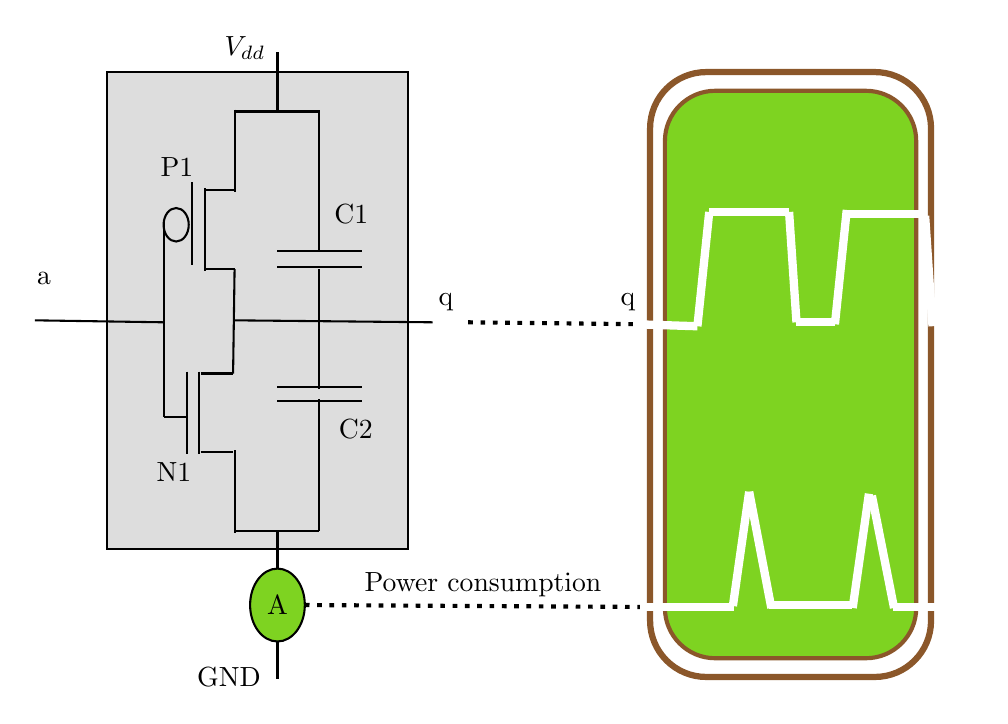
\begin{tikzpicture}[x=0.75pt,y=0.75pt,yscale=-1,xscale=1]
%uncomment if require: \path (0,335); %set diagram left start at 0, and has height of 335

%Shape: Rectangle [id:dp0360003318411668] 
\draw  [fill={rgb, 255:red, 207; green, 207; blue, 207 }  ,fill opacity=0.71 ] (39.45,26.06) -- (184.07,26.06) -- (184.07,255.79) -- (39.45,255.79) -- cycle ;
%Straight Lines [id:da9130268694115924] 
\draw    (4.54,145.67) -- (66.52,146.62) ;


%Straight Lines [id:da1343440150952362] 
\draw    (66.52,98.21) -- (66.52,192.18) ;


%Shape: Ellipse [id:dp6213874655305351] 
\draw   (72.57,91.56) .. controls (75.92,91.56) and (78.63,95.17) .. (78.63,99.63) .. controls (78.63,104.09) and (75.92,107.7) .. (72.57,107.7) .. controls (69.23,107.7) and (66.52,104.09) .. (66.52,99.63) .. controls (66.52,95.17) and (69.23,91.56) .. (72.57,91.56) -- cycle ;
%Straight Lines [id:da27434486206672837] 
\draw    (66.52,192.18) -- (77.2,192.18) ;


%Straight Lines [id:da07016771982069758] 
\draw    (77.92,170.35) -- (77.92,210.22) ;


%Straight Lines [id:da19036973562649373] 
\draw    (83.62,170.35) -- (83.62,210.22) ;


%Straight Lines [id:da8345791716423674] 
\draw    (80.05,79.22) -- (80.05,119.09) ;


%Straight Lines [id:da3271159414725533] 
\draw    (86.47,82.07) -- (86.47,121.94) ;


%Straight Lines [id:da14873596785352006] 
\draw    (84.33,209.27) -- (100,209.27) ;


%Straight Lines [id:da4420681124736481] 
\draw    (84.33,171.3) -- (100,171.3) ;


%Straight Lines [id:da04393107109208283] 
\draw    (87.18,120.99) -- (100.72,120.99) ;


%Straight Lines [id:da3871143133174997] 
\draw    (87.18,83.02) -- (100.72,83.02) ;


%Straight Lines [id:da5151381716842007] 
\draw    (100.72,120.99) -- (100,171.3) ;


%Straight Lines [id:da6069121794097094] 
\draw    (100.72,44.1) -- (100.72,83.97) ;


%Straight Lines [id:da2848668560084322] 
\draw    (100.72,208.32) -- (100.72,248.19) ;


%Straight Lines [id:da29161700195638374] 
\draw    (101.43,45.05) -- (142.04,45.05) ;


%Straight Lines [id:da2980631065657684] 
\draw    (100.72,247.24) -- (141.32,247.24) ;


%Straight Lines [id:da3565336880454746] 
\draw    (141.32,45.05) -- (141.32,112.45) ;


%Straight Lines [id:da47251450500555436] 
\draw    (141.32,183.64) -- (141.32,247.24) ;


%Straight Lines [id:da3833560512127223] 
\draw    (121.38,184.59) -- (161.98,184.59) ;


%Straight Lines [id:da8160698305270608] 
\draw    (121.38,177.95) -- (161.98,177.95) ;


%Straight Lines [id:da053729746303400994] 
\draw    (121.38,112.45) -- (161.98,112.45) ;


%Straight Lines [id:da6110612216423352] 
\draw    (121.38,120.04) -- (161.98,120.04) ;


%Straight Lines [id:da24663417263394583] 
\draw    (141.32,120.99) -- (141.32,178.9) ;


%Straight Lines [id:da6538334507705081] 
\draw    (100.72,145.67) -- (196.18,146.62) ;


%Straight Lines [id:da6610435045454974] 
\draw    (121.38,16.57) -- (121.38,46) ;


%Straight Lines [id:da11217271094658177] 
\draw    (121.38,247.24) -- (121.38,265.28) ;


%Shape: Ellipse [id:dp5116375931959476] 
\draw  [fill={rgb, 255:red, 126; green, 211; blue, 33 }  ,fill opacity=1 ] (108.2,282.84) .. controls (108.2,273.14) and (114.1,265.28) .. (121.38,265.28) .. controls (128.65,265.28) and (134.56,273.14) .. (134.56,282.84) .. controls (134.56,292.54) and (128.65,300.4) .. (121.38,300.4) .. controls (114.1,300.4) and (108.2,292.54) .. (108.2,282.84) -- cycle ;
%Straight Lines [id:da9407053227115245] 
\draw    (121.38,300.4) -- (121.38,318.44) ;


%Rounded Rect [id:dp5069309881092712] 
\draw  [color={rgb, 255:red, 139; green, 87; blue, 42 }  ,draw opacity=1 ][line width=2.25]  (300.91,53.14) .. controls (300.91,38.18) and (313.03,26.06) .. (327.98,26.06) -- (409.2,26.06) .. controls (424.15,26.06) and (436.27,38.18) .. (436.27,53.14) -- (436.27,290.42) .. controls (436.27,305.37) and (424.15,317.49) .. (409.2,317.49) -- (327.98,317.49) .. controls (313.03,317.49) and (300.91,305.37) .. (300.91,290.42) -- cycle ;
%Rounded Rect [id:dp10813466593651544] 
\draw  [color={rgb, 255:red, 139; green, 87; blue, 42 }  ,draw opacity=1 ][fill={rgb, 255:red, 126; green, 211; blue, 33 }  ,fill opacity=1 ][line width=1.5]  (308.05,59.3) .. controls (308.05,45.92) and (318.89,35.08) .. (332.27,35.08) -- (404.91,35.08) .. controls (418.29,35.08) and (429.13,45.92) .. (429.13,59.3) -- (429.13,284.26) .. controls (429.13,297.63) and (418.29,308.47) .. (404.91,308.47) -- (332.27,308.47) .. controls (318.89,308.47) and (308.05,297.63) .. (308.05,284.26) -- cycle ;
%Straight Lines [id:da10126802822138314] 
\draw [line width=1.5]  [dash pattern={on 1.69pt off 2.76pt}]  (213.28,146.62) -- (298.77,147.57) ;


%Straight Lines [id:da8166666674599945] 
\draw [line width=1.5]  [dash pattern={on 1.69pt off 2.76pt}]  (134.56,282.84) -- (301.26,283.79) ;


%Straight Lines [id:da6599388820944971] 
\draw [color={rgb, 255:red, 255; green, 255; blue, 255 }  ,draw opacity=1 ][line width=3]    (294.5,147.57) -- (323.71,148.52) ;


%Straight Lines [id:da6477850565472385] 
\draw [color={rgb, 255:red, 255; green, 255; blue, 255 }  ,draw opacity=1 ][line width=3]    (323.71,148.52) -- (329.41,93.46) ;


%Straight Lines [id:da6713764130615041] 
\draw [color={rgb, 255:red, 255; green, 255; blue, 255 }  ,draw opacity=1 ][line width=3]    (329.41,93.46) -- (367.88,93.46) ;


%Straight Lines [id:da6265334534856528] 
\draw [color={rgb, 255:red, 255; green, 255; blue, 255 }  ,draw opacity=1 ][line width=3]    (371.44,146.62) -- (367.88,93.46) ;


%Straight Lines [id:da7580446433818473] 
\draw [color={rgb, 255:red, 255; green, 255; blue, 255 }  ,draw opacity=1 ][line width=3]    (371.44,146.62) -- (389.96,146.62) ;


%Straight Lines [id:da12760629606366103] 
\draw [color={rgb, 255:red, 255; green, 255; blue, 255 }  ,draw opacity=1 ][line width=3]    (389.96,147.57) -- (395.66,92.51) ;


%Straight Lines [id:da35722507690924] 
\draw [color={rgb, 255:red, 255; green, 255; blue, 255 }  ,draw opacity=1 ][line width=3]    (394.95,94.41) -- (433.42,94.41) ;


%Straight Lines [id:da9407492544795262] 
\draw [color={rgb, 255:red, 255; green, 255; blue, 255 }  ,draw opacity=1 ][line width=3]    (436.98,148.52) -- (433.42,95.36) ;


%Straight Lines [id:da36688349354965344] 
\draw [color={rgb, 255:red, 255; green, 255; blue, 255 }  ,draw opacity=1 ][line width=3]    (296.28,283.79) -- (341.16,283.79) ;


%Straight Lines [id:da07990995883843] 
\draw [color={rgb, 255:red, 255; green, 255; blue, 255 }  ,draw opacity=1 ][line width=3]    (340.8,283.31) -- (348.64,228.26) ;


%Straight Lines [id:da7808057757591158] 
\draw [color={rgb, 255:red, 255; green, 255; blue, 255 }  ,draw opacity=1 ][line width=3]    (359.33,284.26) -- (348.64,228.26) ;


%Straight Lines [id:da6401094233638194] 
\draw [color={rgb, 255:red, 255; green, 255; blue, 255 }  ,draw opacity=1 ][line width=3]    (358.26,282.84) -- (398.16,282.84) ;


%Straight Lines [id:da0933201425519079] 
\draw [color={rgb, 255:red, 255; green, 255; blue, 255 }  ,draw opacity=1 ][line width=3]    (398.51,284.26) -- (406.35,229.21) ;


%Straight Lines [id:da038966229239766115] 
\draw [color={rgb, 255:red, 255; green, 255; blue, 255 }  ,draw opacity=1 ][line width=3]    (418.46,284.26) -- (407.77,230.16) ;


%Straight Lines [id:da29582365028992696] 
\draw [color={rgb, 255:red, 255; green, 255; blue, 255 }  ,draw opacity=1 ][line width=3]    (418.1,283.79) -- (458,283.79) ;



% Text Node
\draw (8.81,125.74) node  [align=left] {a};
% Text Node
\draw (72.93,71.63) node  [align=left] {P1};
% Text Node
\draw (71.51,218.76) node  [align=left] {N1};
% Text Node
\draw (157,94.41) node  [align=left] {C1};
% Text Node
\draw (159.13,197.88) node  [align=left] {C2};
% Text Node
\draw (121.38,282.84) node  [align=left] {A};
% Text Node
\draw (202.59,137.13) node  [align=left] {q};
% Text Node
\draw (290.22,137.13) node  [align=left] {q};
% Text Node
\draw (220.4,272.87) node  [align=left] {Power consumption};
% Text Node
\draw (97.99,317.74) node  [align=left] {GND};
% Text Node
\draw (105.7,14.67) node  [align=left] {$\displaystyle V_{dd}$};


\end{tikzpicture}
    \caption{Not gate connected to an oscilloscope.} \label{fig:Not gate connected to an oscilloscope}
\end{figure}

This is the NOT gate as before connected with an ampere meter so we can measure the power consumption, also there are two capacitors (C1 \& C2). The capacitors are connected because the characteristics of the circuit which make it to act like capacitors. They are not transferring current but they will have an effect on the math we are going to do next.

Next we are taking a square wave, which looks like this:

And we have to feed it into the NOT gates, the output is going to be the opposite of the square wave, and we want to measure the power consumption using an oscilloscope. The x axis of the oscilloscope is time and the y axis in this case it's a voltage of the power. It's a current moving across the ampere meter. What we can see here is that when the circuit is stable, there was not much power consumption, but when the system is switching, when there is a high power consumption, because there is a glitch when one transistor is opening and the other one is closing. Also, we can see that the lines in the oscilloscope are not having the same size as the capacitors are actually charging and discharging without we want it. We can learn from this if there was one or zero and what is the rate of switching, and we can store this information.

The power consumption is the sum of the statistic and the dynamic power consumption: 

\begin{displaymath}
    P(t)=P_{stat}(t) + P_{dyn}(t)
\end{displaymath}

We don't care about the statistic power consumption as it is just defined by the kind of silicone that we are using, the size of the features decided to be in the transistors, the temperature, the technology, etc. But really interesting for us is the dynamic power consumption that depends on the o'clock rate and the circuit activity input data.

Because the power consumption is a function of the circuit activity, we can try to measure the power consumption and send the results to the equations and to get the circuit activity, in a way we can find out all the secrets.

In order to calculate the power consumption this way we need a lots of data about the circuit and about the environment and about the temperature etc. And this is too much work for us as an engineers. There is a much simplified way of measuring the power consumption of a device, assuming it's a CMOS device we can measure how many bits changes every clock.

So, our assumptions are the followings:
\begin{inparaenum}
    \item This is a CMOS device.
    \item When it's static the static power is very low, and when it switches, there is a very high power consumption.
    \item This is synchronous circuit, which means it has a lot of flip flops that all change at the same time.
    \item The power consumption is proportional to the amount of changes and the outputs of these flip flops.
\end{inparaenum}


\subsection { hamming distance model }

For doing this we are going to use hamming distance model. The Hamming distance between two vectors is the number of bits we must change to change one into the other. Example, what is the distance between the vectors 01101010 and 11011011? 

Answer: They differ in four places, so the Hamming distance d(01101010,11011011) = 4.

When talking about CMOS devices we are estimating our power consumption as amount of bits (transitions) that change from one to zero or from zero to one, this is our hamming distance. By monitoring the changes as explained we can find the power consumption.

But, this is not enough. By connecting the oscilloscope to our device we are trying to measure a physical device with another physical equipment, and what they are measuring is subject to measurement errors like switching noise, thermal noise and measurement noises.

Switching noise means that there are other kinds of activity which are going on in the circuit in addition. Measurement noise means that our desk setup is not always accurate, or we might be connected not properly, or we might not be measuring the precise correct moment of time etc. Thermal noise - we are measuring electrical activity, as electrons are very crazy particles and they like to disappear and reappear in a nearby location. So the higher is the temperature, the more likely they are to vanish and disappear. And when the electrons are moving, they generate radiation and they affect our measurements.

So now when we are measuring the power, we get the static power, the dynamic power and we get the noise:

\begin{displaymath}
    P_{meas}(t)=P_{stat}(t) + P_{dyn}(t) + N(t)
\end{displaymath}

In order to avoid the noise we can measure it again and again and then the noise might be canceling itself. What happens sometimes is that the noise, especially the switching noise, is sometimes correlated with the activity of the circuits. Another thing we can do is controlling the noise somehow like running our experiment inside a freezer, or an isolated environment where there's no electric noise around. We can also, open the dives and try to kill the sources of noise.

That's one very nice thing we can do is instead of measuring power consumption, we can measure electromagnetic radiation. And this has two advantages, first of all, it's less invasive and second of all, it can be focused and, and reduce the switching noise.

\subsection { From Power to Electromagnetic }

\begin{figure}[!ht]
    \centering
    \tikzset{every picture/.style={line width=0.75pt}} %set default line width to 0.75pt        

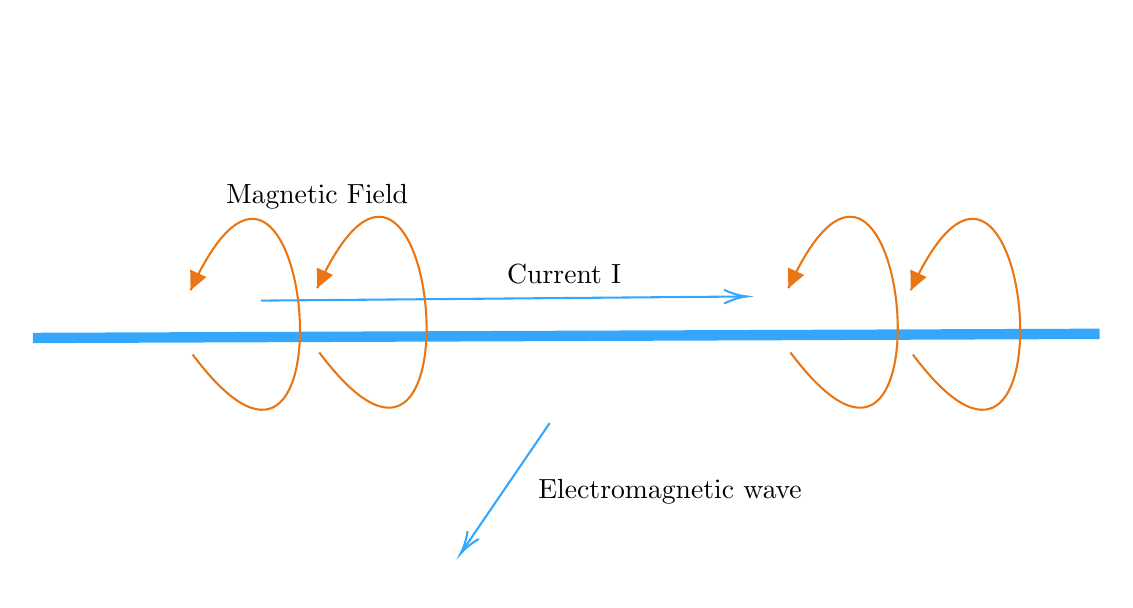
\begin{tikzpicture}[x=0.75pt,y=0.75pt,yscale=-1,xscale=1]
%uncomment if require: \path (0,300); %set diagram left start at 0, and has height of 300

%Straight Lines [id:da730115903310417] 
\draw [color={rgb, 255:red, 52; green, 167; blue, 252 }  ,draw opacity=1 ][line width=3.75]    (69,171) -- (583,169) ;


%Straight Lines [id:da8949672238779289] 
\draw [color={rgb, 255:red, 52; green, 167; blue, 252 }  ,draw opacity=1 ]   (179,153) -- (411,151.02) ;
\draw [shift={(413,151)}, rotate = 539.51] [color={rgb, 255:red, 52; green, 167; blue, 252 }  ,draw opacity=1 ][line width=0.75]    (10.93,-3.29) .. controls (6.95,-1.4) and (3.31,-0.3) .. (0,0) .. controls (3.31,0.3) and (6.95,1.4) .. (10.93,3.29)   ;

%Curve Lines [id:da4084322101826783] 
\draw [color={rgb, 255:red, 233; green, 117; blue, 20 }  ,draw opacity=1 ]   (493,179) .. controls (574,287) and (549,23) .. (492,148) ;
\draw [shift={(492,148)}, rotate = 294.51] [fill={rgb, 255:red, 233; green, 117; blue, 20 }  ,fill opacity=1 ][line width=0.75]  [draw opacity=0] (8.93,-4.29) -- (0,0) -- (8.93,4.29) -- cycle    ;

%Straight Lines [id:da8207423009134964] 
\draw [color={rgb, 255:red, 52; green, 167; blue, 252 }  ,draw opacity=1 ]   (318,212) -- (276.13,273.35) ;
\draw [shift={(275,275)}, rotate = 304.32] [color={rgb, 255:red, 52; green, 167; blue, 252 }  ,draw opacity=1 ][line width=0.75]    (10.93,-3.29) .. controls (6.95,-1.4) and (3.31,-0.3) .. (0,0) .. controls (3.31,0.3) and (6.95,1.4) .. (10.93,3.29)   ;

%Curve Lines [id:da43215348815507637] 
\draw [color={rgb, 255:red, 233; green, 117; blue, 20 }  ,draw opacity=1 ]   (434,178) .. controls (515,286) and (490,22) .. (433,147) ;
\draw [shift={(433,147)}, rotate = 294.51] [fill={rgb, 255:red, 233; green, 117; blue, 20 }  ,fill opacity=1 ][line width=0.75]  [draw opacity=0] (8.93,-4.29) -- (0,0) -- (8.93,4.29) -- cycle    ;

%Curve Lines [id:da7658292921428724] 
\draw [color={rgb, 255:red, 233; green, 117; blue, 20 }  ,draw opacity=1 ]   (146,179) .. controls (227,287) and (202,23) .. (145,148) ;
\draw [shift={(145,148)}, rotate = 294.51] [fill={rgb, 255:red, 233; green, 117; blue, 20 }  ,fill opacity=1 ][line width=0.75]  [draw opacity=0] (8.93,-4.29) -- (0,0) -- (8.93,4.29) -- cycle    ;

%Curve Lines [id:da6169102709245924] 
\draw [color={rgb, 255:red, 233; green, 117; blue, 20 }  ,draw opacity=1 ]   (207,178) .. controls (288,286) and (263,22) .. (206,147) ;
\draw [shift={(206,147)}, rotate = 294.51] [fill={rgb, 255:red, 233; green, 117; blue, 20 }  ,fill opacity=1 ][line width=0.75]  [draw opacity=0] (8.93,-4.29) -- (0,0) -- (8.93,4.29) -- cycle    ;


% Text Node
\draw (206,103) node  [align=left] {Magnetic Field};
% Text Node
\draw (325,140) node  [align=left] {Current I};
% Text Node
\draw (376,245) node  [align=left] {Electromagnetic wave};


\end{tikzpicture}


    \caption{electromagnetic emission.} \label{fig:electromagnetic emission}
\end{figure}

Electric fields are created by differences in voltage: the higher the voltage, the stronger will be the resultant field. We can use the right hand rule in order to remember the direction of the electromagnetic field direction when we know the current direction. We can measure the magnetic field, but one disadvantage is that it is very localize, so we need to get access to the device. We can connect an antenna to the device and then we can measure the electromagnetic wave using a receiver. There is a very nice paper called screaming channels where you can read more about this kind of attacks.